\chapterimage{head2.png} % Chapter heading image
\chapter{Bayesian Inference Framework}
\section{Graphical Model}
\begin{definition}
We denote a particular configuration as $(\textbf{x}, \textbf{y})$
\begin{equation}
(\textbf{x}, \textbf{y})=(x_0, x_1, \cdots, x_T, y_1, \cdots, y_T)
\end{equation}
\end{definition}

\begin{definition}[The joint probability]
\begin{equation}
p(\textbf{x}, \textbf{y})= p(x_0)\prod_{t=0}^{T-1} p(x_{t+1}|x_t) \prod_{t=0}^{T}p(y_t|x_t)
\end{equation}
\end{definition}
\begin{center}
        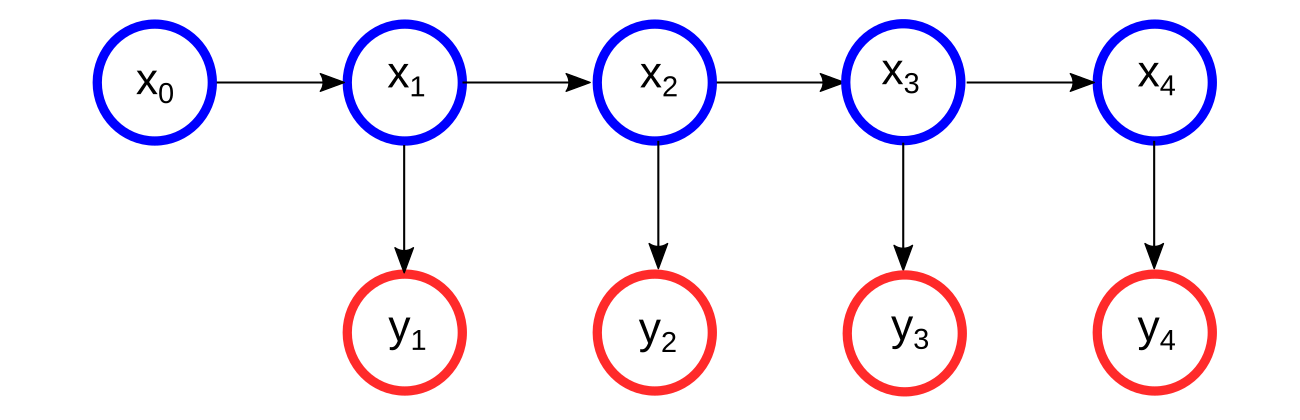
\includegraphics[scale=0.8]{ch2/four_states_ex.png}   
\end{center}

\section{Forward algorithm}
\subsection{Probability Meaning}
$ \left<\alpha_{t_{\tau}}|x \right>$ is the joint probability amplitude of emitting a partial sequence of outputs $(y_1,\cdots,y_{\tau})$ and ending up in state $x_{\tau}$. That is,
\begin{equation}
        (\left<\alpha_{t_{\tau}}|x \right>)^2 = p(y_1,\cdots,y_{\tau}, x_{\tau})
\end{equation}
For example, $(\left<\alpha_{t_2}|x \right>)^2 = p(y_1, y_2, x_2)$
\begin{center}
        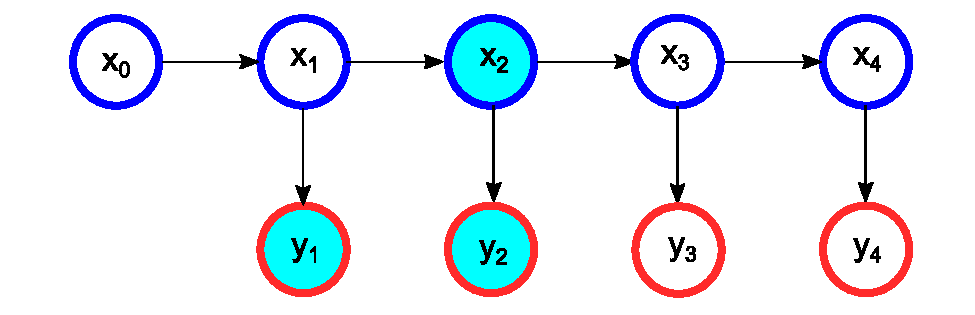
\includegraphics[scale=0.8]{ch2/alpha_example.pdf}
\end{center}
\subsection{alpha-t0}
\begin{definition}[$\left< \hat{\alpha}_{t_0} \right|$]
Since there is no external forces, the initial state, $\left< \alpha_{t_0} \right|$, is assumed to follow the equilibrium distribution $\rho_{eq}(x)=\sqrt{p_{eq}(x)}$, that is
\begin{equation}
        \left< \alpha_{t_0} | x \right> = \rho_{eq}(x)
\end{equation}
\begin{center}
        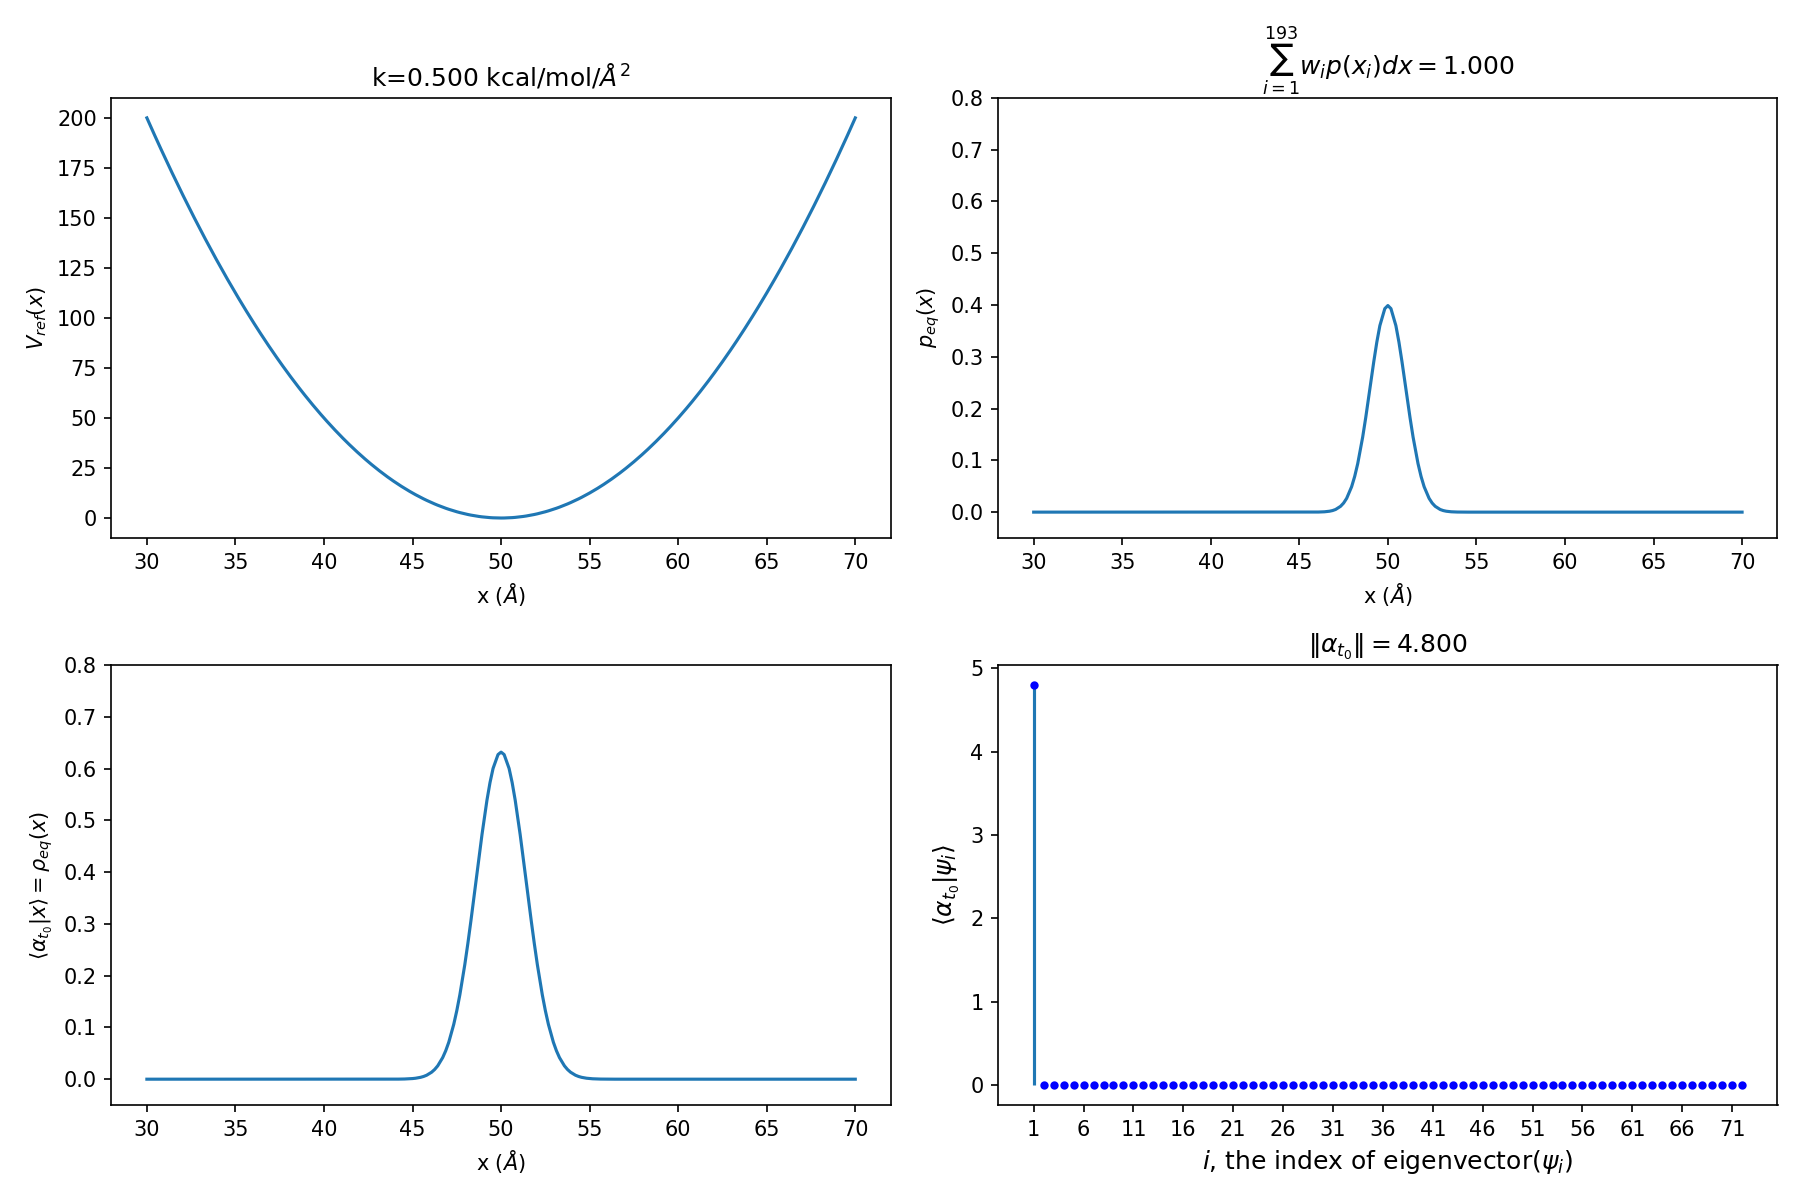
\includegraphics[scale=0.45]{ch2/alpha_t0.png}   
\end{center}
And we know
\begin{align*}
        p(x,t=0) &= \rho_{eq}(x) \rho_{eq}(x)\\
        &= \rho_{eq}(x)[\left< \alpha_{t_0} | \psi_1 \right> \psi_1(x) + \left< \alpha_{t_0} | \psi_2 \right>\psi_2(x)+\cdots+\left< \alpha_{t_0} | \psi_{72} \right>\psi_{72}(x)]       
\end{align*}
where
\begin{align*}
        \left< \alpha_{t_0} | \psi_j \right> = \int w(x) \rho_{eq}(x) \psi_j(x) dx \approx \sum_{i=1}^{193} w(x_i) \rho_{eq}(x_i) \psi_j(x_i)
\end{align*}
$\left< \alpha_{t_0} \right|$ is a vector, which is shown in the right-bottom figure.
\begin{equation}
        \left< \alpha_{t_0} \right| = \begin{bmatrix}\left< \alpha_{t_0} | \psi_1 \right> & \left< \alpha_{t_0} | \psi_2 \right> & \cdots & \left< \alpha_{t_0} | \psi_{72} \right> \end{bmatrix}
\end{equation}
and the norm of $\left< \alpha_{t_0} \right|$ is defined by
\begin{align}
        \norm{\alpha_{t_0}} &=  \sqrt{\int w(x) (\left< \alpha_{t_0} | x_i \right>)^2 dx} \approx \sqrt{ \sum_{i=1}^{193} w(x_i) (\left< \alpha_{t_0} | x_i \right>)^2 } \\
        \norm{\alpha_{t_0}} &= \sqrt{(\left< \alpha_{t_0} | \psi_1 \right>)^2 + (\left< \alpha_{t_0} | \psi_2 \right>)^2 +\cdots + (\left< \alpha_{t_0} | \psi_{72} \right>)^2}
\end{align}
Furthermore, note that
\begin{equation}
        \left< \hat{\alpha}_{t_0} \right| = \frac{\left< \alpha_{t_{0}} \right|}{\norm{\alpha_{t_{0}}}} = \left< \alpha_{t_{0}} \right|
\end{equation}
because $\norm{\alpha_{t_0}} = 1$
\end{definition}

\begin{definition}[$\rho(x, t=\Delta t) = \left<\alpha_{t_0}| e^{-\textbf{H}\Delta t}|x \right>$]
\begin{align*}
        &p(x,t=\Delta t) = \rho_{eq}(x) \rho(x, \Delta t)\\
        &= \rho_{eq}(x)[ \left< \alpha_{t_0} | \psi_1 \right> e^{-\lambda_{1}\Delta t}\psi_1(x) + \cdots+ \left< \alpha_{t_0} | \psi_{72} \right> e^{(-\lambda_{72}\Delta t)}\psi_{72}(x)]  \\
        &=  \rho_{eq}(x)[ \left< \alpha_{t_0} | \psi_1 \right>\psi_1(x)+ \cdots + \left< \alpha_{t_0} | \psi_{72} \right> e^{(-\lambda_{72}\Delta t)}\psi_{72}(x)]  
\end{align*}
where $\lambda_1 = 0$
\begin{center}
        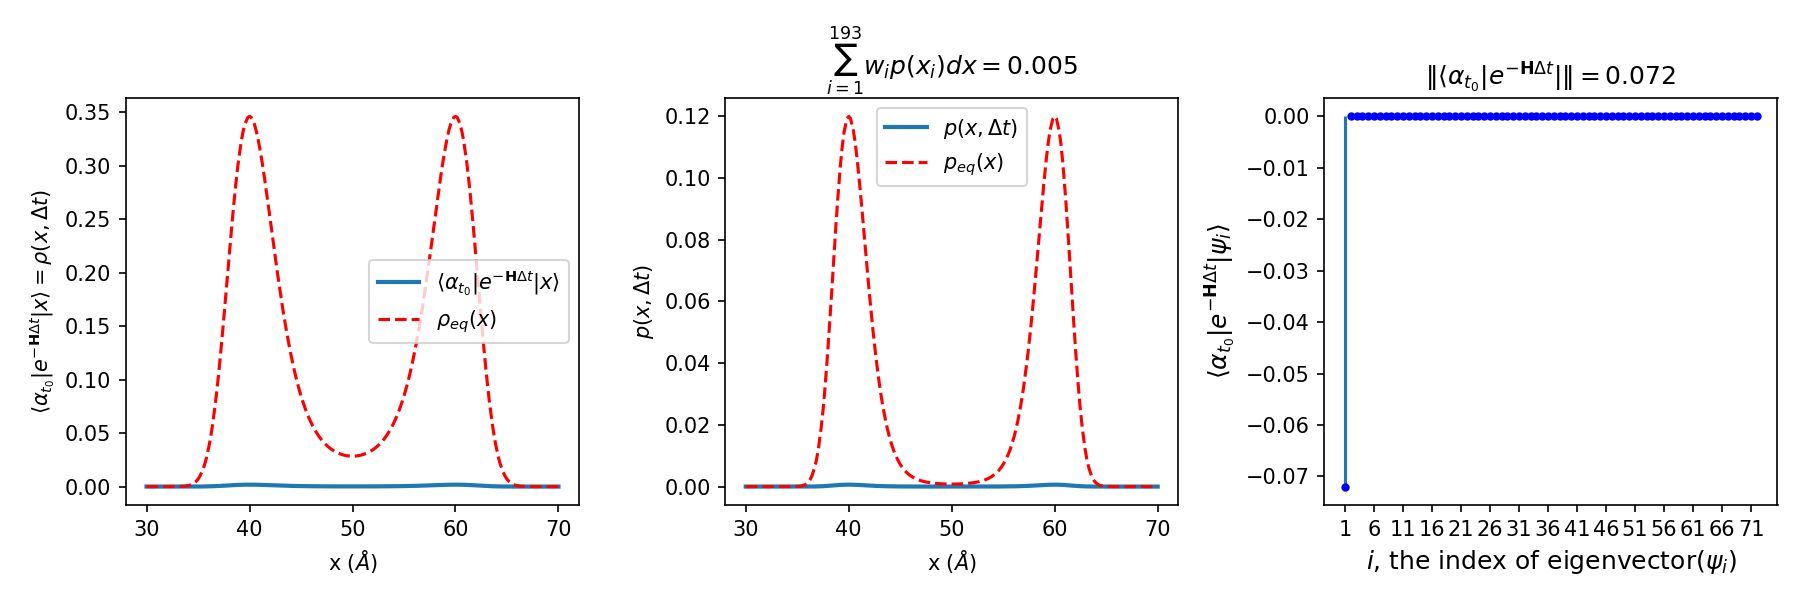
\includegraphics[scale=0.35]{ch2/alpha_t0_exp_dt.png}   
\end{center}
\end{definition}

\subsection{alpha-t1}
\begin{definition}[$\left< \hat{\alpha}_{t_1}\right|$]
\begin{equation}
        \left< \alpha_{t_1} \right| = \left< \alpha_{t_0} \right| e^{-\textbf{H} \Delta t} \textbf{y}_1     
\end{equation}
\begin{center}
        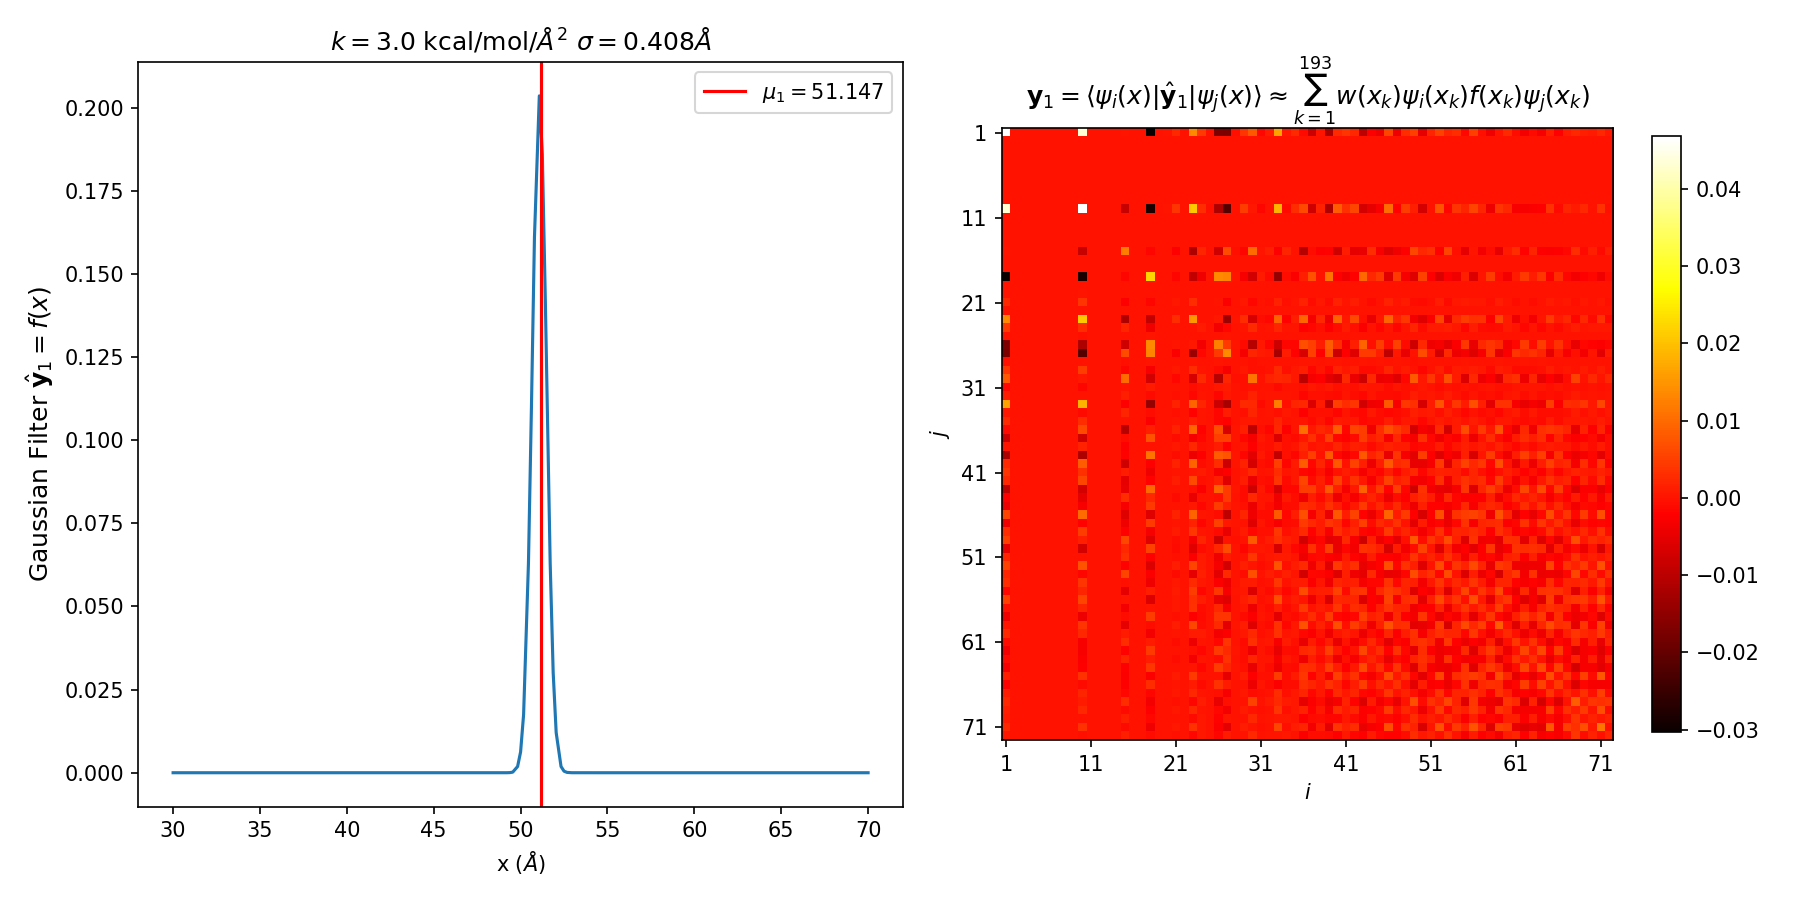
\includegraphics[scale=0.25]{ch2/photon_operator_y1.png}   
\end{center}
$\left< \alpha_{t_1} \right|$ carries "the joint probability amplitude" of observing all the photon data during $[0, t_1]$ and the system state at $t_1$, that is
\begin{equation}
        p(x, y_1) = (\left< \alpha_{t_1} | x \right>)^2
\end{equation}
We can do normalization to get $\left< \hat{\alpha}_{t_1} \right|$.
\begin{equation}
        \left< \hat{\alpha}_{t_1} \right| = \frac{\left< \alpha_{t_0} \right| e^{-\textbf{H}\Delta t} \textbf{y}_1}{\norm{\left< \alpha_{t_0} \right| e^{-\textbf{H}\Delta t} \textbf{y}_1}} = \frac{\left< \alpha_{t_{1}} \right|}{\norm{\alpha_{t_{1}}}}
\end{equation}
\begin{center}
        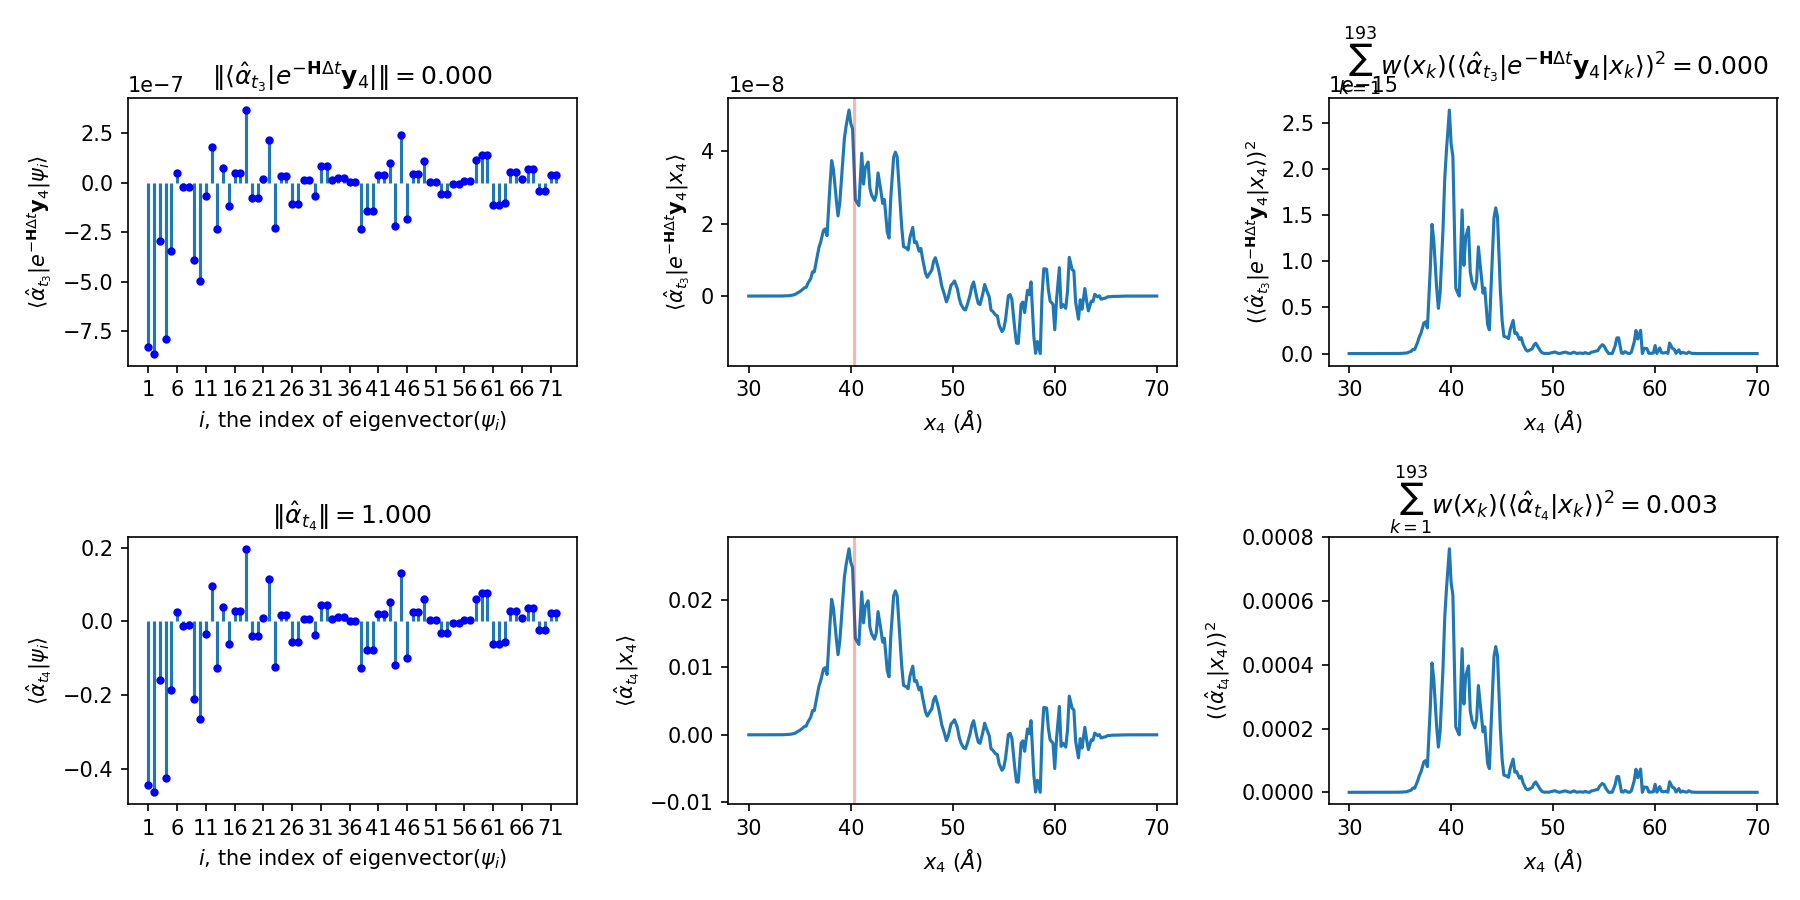
\includegraphics[scale=0.4]{ch2/alpha_1.png}   
\end{center}
$\left< \hat{\alpha}_{t_1} \right|$ is a probability amplitude, which square is 
\begin{align*}
        p(x | y_1) =  (\left< \hat{\alpha}_{t_1} | x \right>)^2
\end{align*}
Therefore
\begin{align*}
        \int p(x|y_1) dx \approx \sum_{k=1}^{193}w(x_k)(\left< \hat{\alpha}_{t_1} | x_k \right>)^2 &= 1 \\
        \norm{\hat{\alpha_{t_1}}} &= 1
\end{align*}
\end{definition}

\begin{definition}[$\left< \hat{\alpha}_{t_1}| e^{-\textbf{H}\Delta t} \right|$]
\begin{align*}
        \left< \hat{\alpha}_{t_1}| e^{-\textbf{H}\Delta t} \right| &= 
        \begin{bmatrix}
                \left< \hat{\alpha}_{t_1}| e^{-\textbf{H}\Delta t} | \psi_1 \right> &
                \left< \hat{\alpha}_{t_1}| e^{-\textbf{H}\Delta t} | \psi_2 \right> & 
                \cdots &
                \left< \hat{\alpha}_{t_1}| e^{-\textbf{H}\Delta t} | \psi_{72} \right>
        \end{bmatrix}\\
        &=
        \begin{bmatrix}
                e^{-\lambda_{1}\Delta t} \left< \hat{\alpha}_{t_1} | \psi_1 \right> &
                e^{-\lambda_{2}\Delta t} \left< \hat{\alpha}_{t_1} | \psi_2 \right> & 
                \cdots &
                e^{-\lambda_{72}\Delta t} \left< \hat{\alpha}_{t_1} | \psi_{72} \right> 
        \end{bmatrix}\\ 
        &=
        \begin{bmatrix}
                \left< \hat{\alpha}_{t_1} | \psi_1 \right> &
                e^{-\lambda_{2}\Delta t} \left< \hat{\alpha}_{t_1} | \psi_2 \right> & 
                \cdots &
                e^{-\lambda_{72}\Delta t} \left< \hat{\alpha}_{t_1} | \psi_{72} \right> 
        \end{bmatrix}
\end{align*}
The probability meaning is 
\begin{align*}
        (\left< \hat{\alpha}_{t_1}| e^{-\textbf{H}\Delta t} | x \right>)^2 = F(x_2) = p(x_1|y_1) p(x_2|x_1) 
\end{align*}
The case in our simulation, when $\Delta t = 10^{-9}$ s 
\begin{center}
        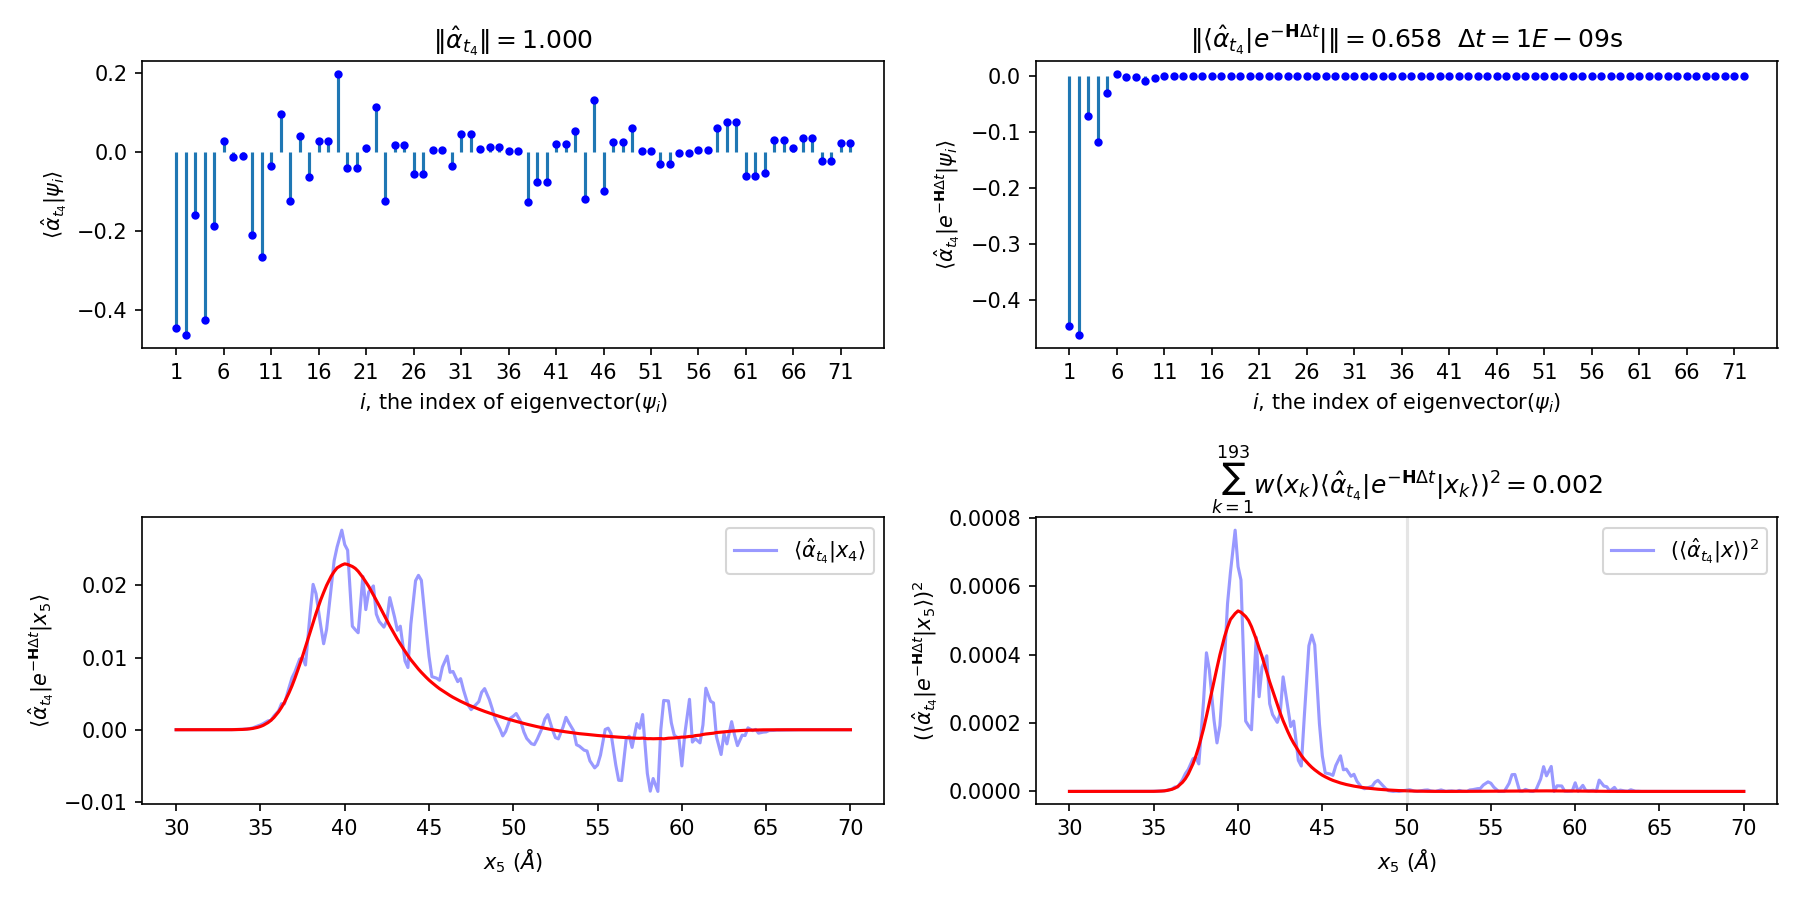
\includegraphics[scale=0.4]{ch2/alphat1_expdt_normalcase.png}   
\end{center}
In the right-bottom figure
\begin{align*}
        \int p(x_1|y_1)p(x_2|x_1)dx_2 = 0.326
\end{align*}
\end{definition}

\subsection{alpha-t2}
\begin{definition}[$\left< \hat{\alpha}_{t_2}\right|$]
\begin{equation}
        \left< \alpha_{t_2} \right| = \left< \alpha_{t_1} \right| e^{-\textbf{H}\Delta t} \textbf{y}_2     
\end{equation}
\begin{center}
        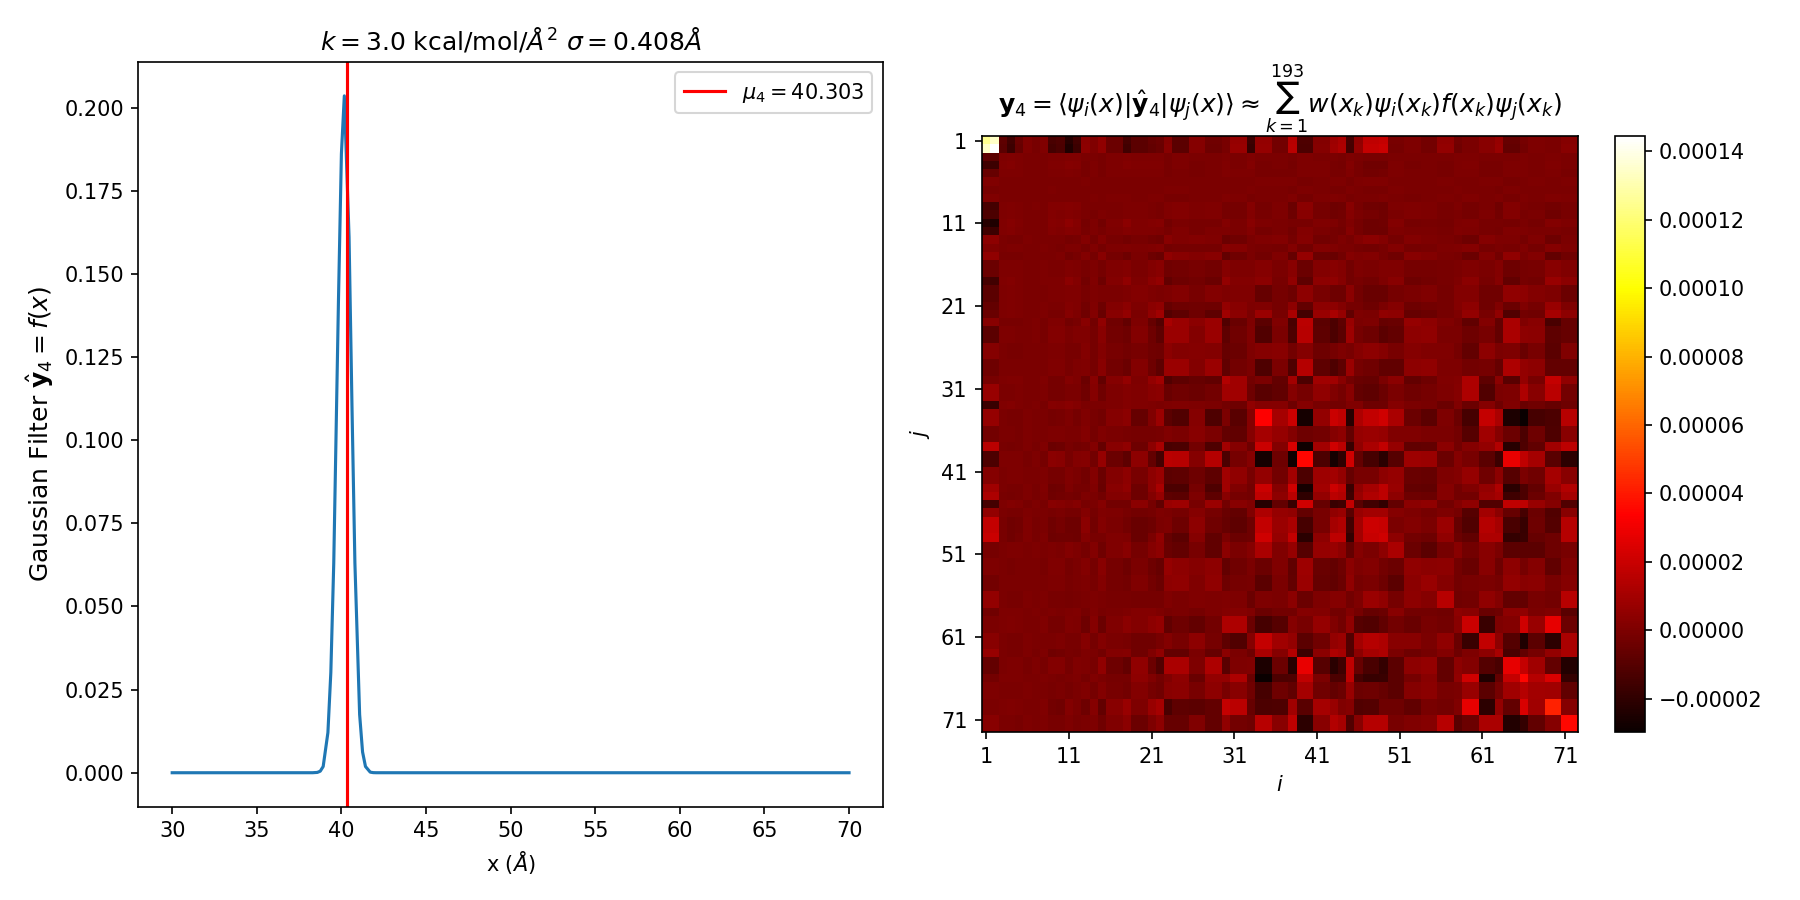
\includegraphics[scale=0.25]{ch2/photon_operator_y2.png}   
\end{center}
The probability meaning for $\left< \alpha_{t_2}\right|$ is 
\begin{align*}
        p(x_2, y_1, y_2) = (\left< \alpha_{t_2}| x \right>)^2
\end{align*}
and we can do normalization to get $\left< \hat{\alpha}_{t_2} \right|$, it has the information
\begin{equation}
        p(x|y_1,y_2) = (\left< \hat{\alpha}_{t_2} |x\right>)^2
\end{equation}
In detail
\begin{equation}
        \left< \hat{\alpha}_{t_2} \right| 
	= \frac{\left< \hat{\alpha}_{t_1} \right| e^{-\textbf{H}\Delta t} \textbf{y}_2}{\norm{\left< \hat{\alpha}_{t_1} \right| e^{-\textbf{H}\Delta t} \textbf{y}_2}} 
	= \frac{1}{\norm{\alpha_{t_{1}}}} \frac{\left< \alpha_{t_1} \right| e^{-\textbf{H}\Delta t} \textbf{y}_2}{\norm{\left< \hat{\alpha}_{t_1} \right| e^{-\textbf{H}\Delta t} \textbf{y}_2}} 
	= \frac{1}{\norm{\alpha_{t_{1}}}} \frac{1}{\norm{\left< \hat{\alpha}_{t_1} \right| e^{-\textbf{H}\Delta t} \textbf{y}_2}} \left< \alpha_{t_2} \right| 
	= \frac{1}{\norm{\alpha_{t_2}}} \left< \alpha_{t_2} \right|
\end{equation}
where
\begin{equation}
        \norm{\alpha_{t_2}} = \norm{\alpha_{t_{1}}} \norm{\left< \hat{\alpha}_{t_1} \right| e^{-\textbf{H}\Delta t} \textbf{y}_2} 
	= \norm{\left < \hat{\alpha}_{t_{0}} \right| e^{-\textbf{H}\Delta t} \textbf{y}_1} \norm{\left< \hat{\alpha}_{t_1} \right| e^{-\textbf{H}\Delta t} \textbf{y}_2}
\end{equation}
\begin{center}
        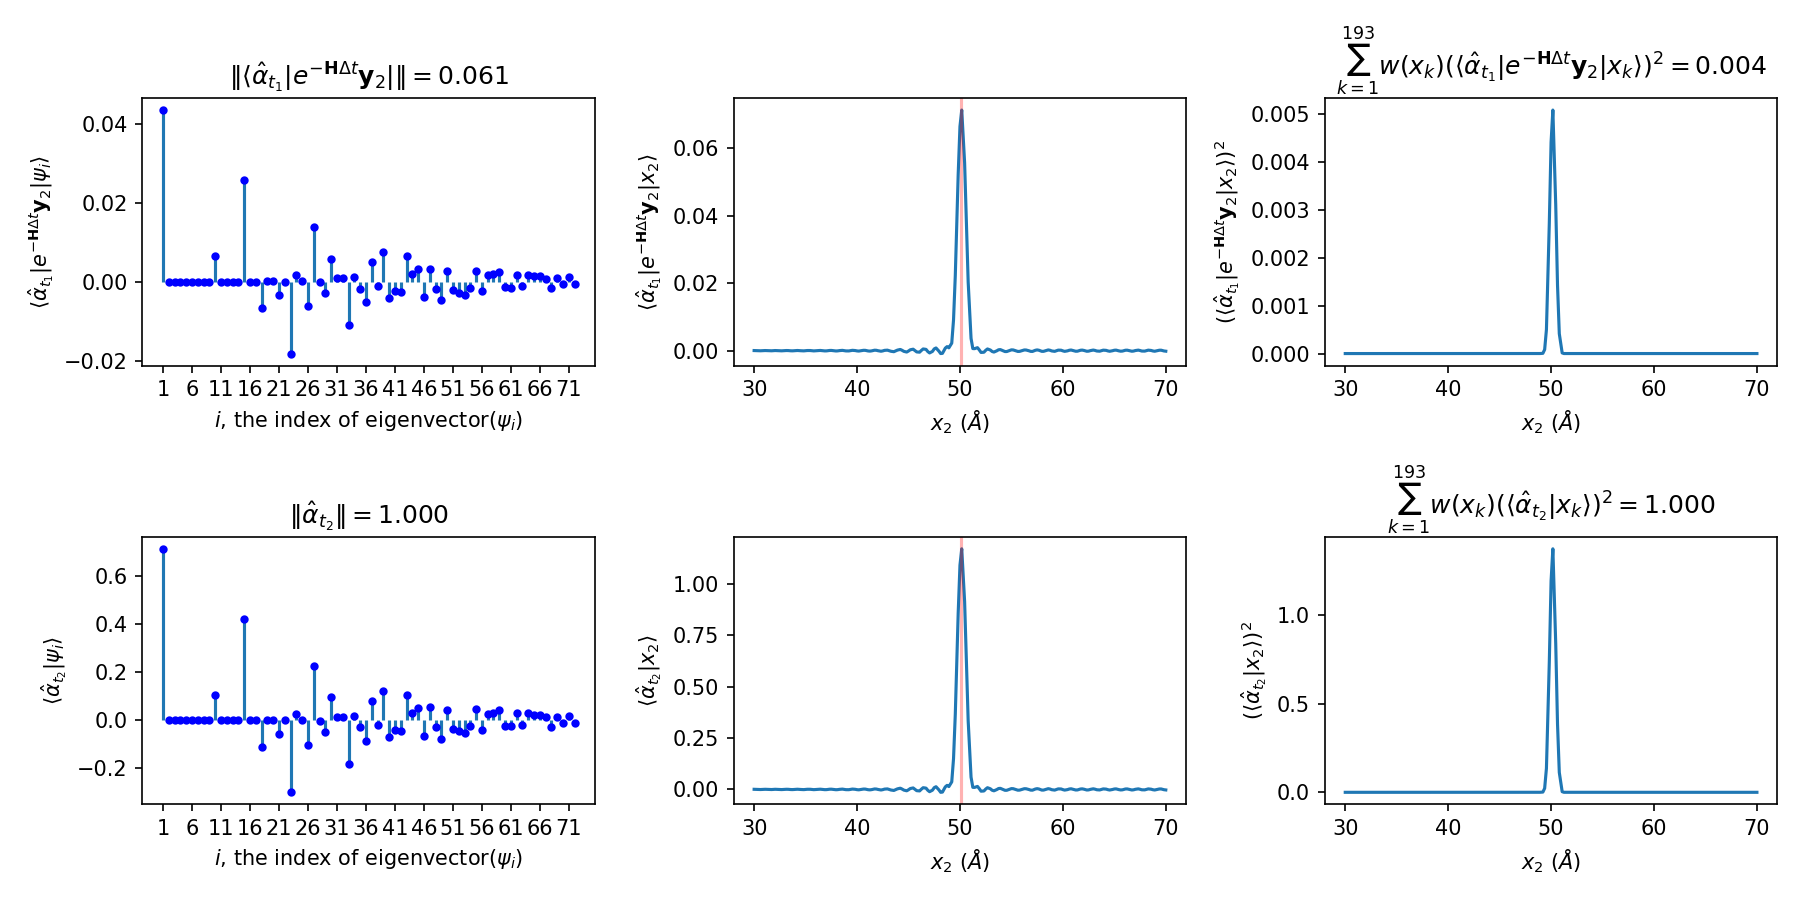
\includegraphics[scale=0.4]{ch2/alpha_2.png}   
\end{center}
\end{definition}

\begin{definition}[$\left< \hat{\alpha}_{t_2}| e^{-\textbf{H}\Delta t} \right|$]
The probability meaning is 
\begin{align*}
        (\left< \hat{\alpha}_{t_2}| e^{-\textbf{H}\Delta t} | x_3 \right>)^2 = \int p(x_2 | y_1, y_2) p(x_3|x_2) dx_3  
\end{align*}
\begin{center}
        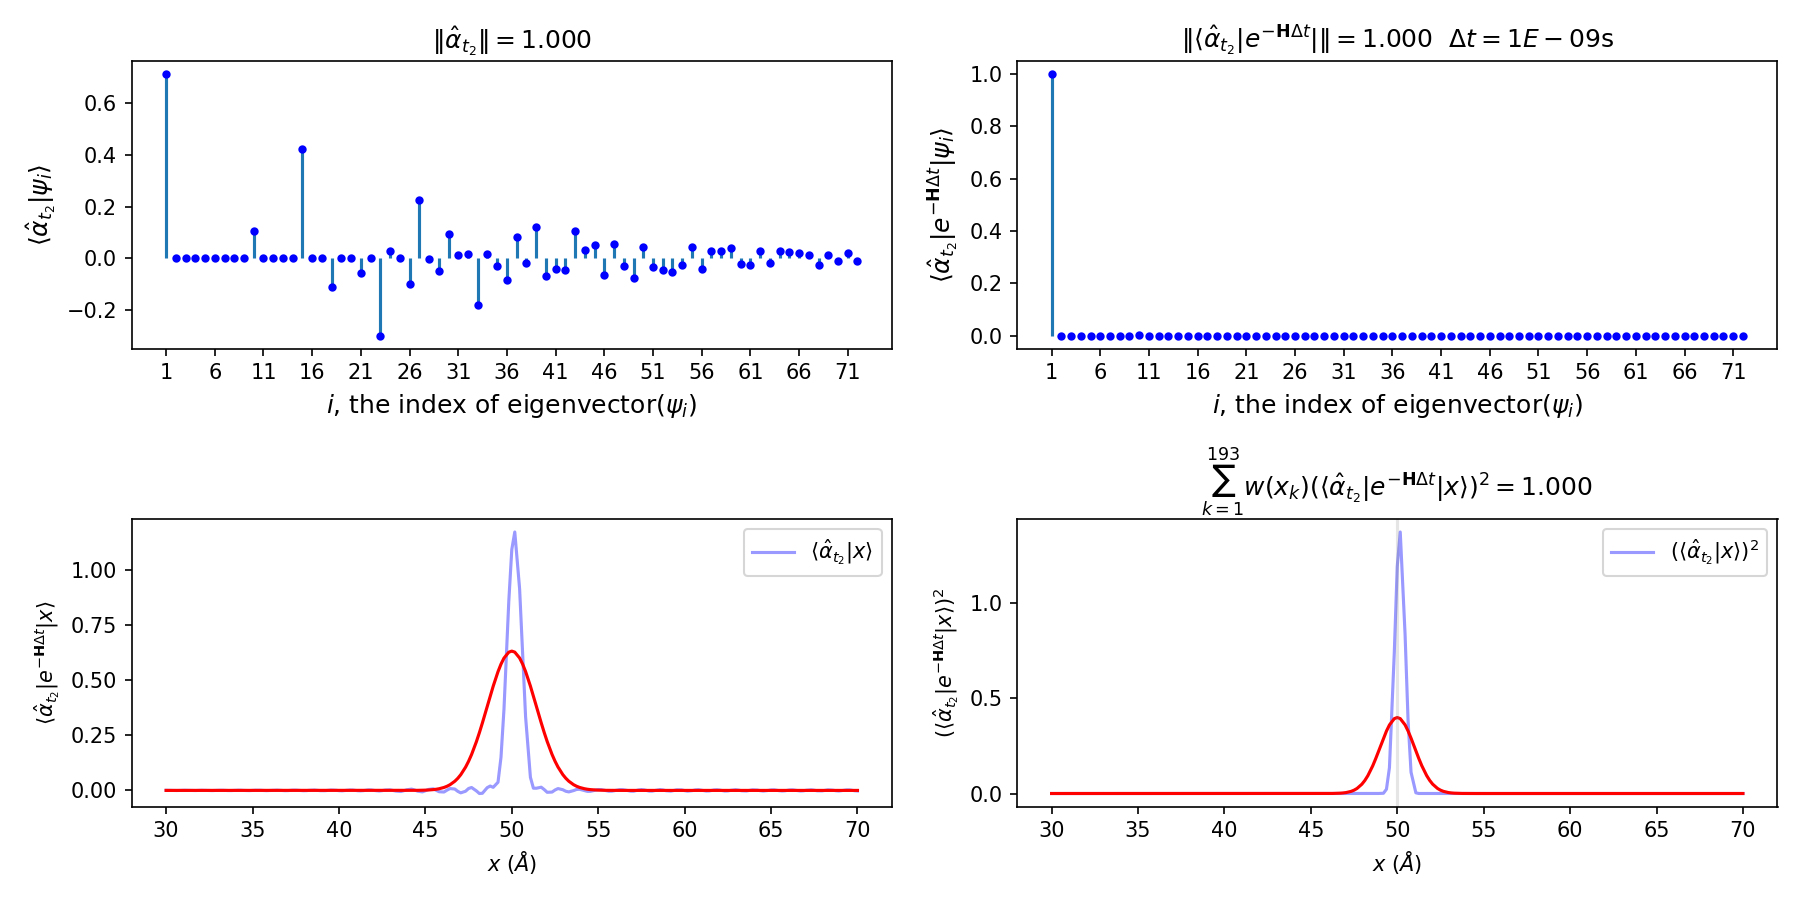
\includegraphics[scale=0.4]{ch2/alphat2_expdt.png}   
\end{center}
\end{definition}

\subsection{alpha-t3}
\begin{definition}[$\left< \hat{\alpha}_{t_3}\right|$]
\begin{equation}
        \left< \alpha_{t_3} \right| = \left< \alpha_{t_2} \right| e^{-\textbf{H}\Delta t} \textbf{y}_3               
\end{equation}
\begin{center}
        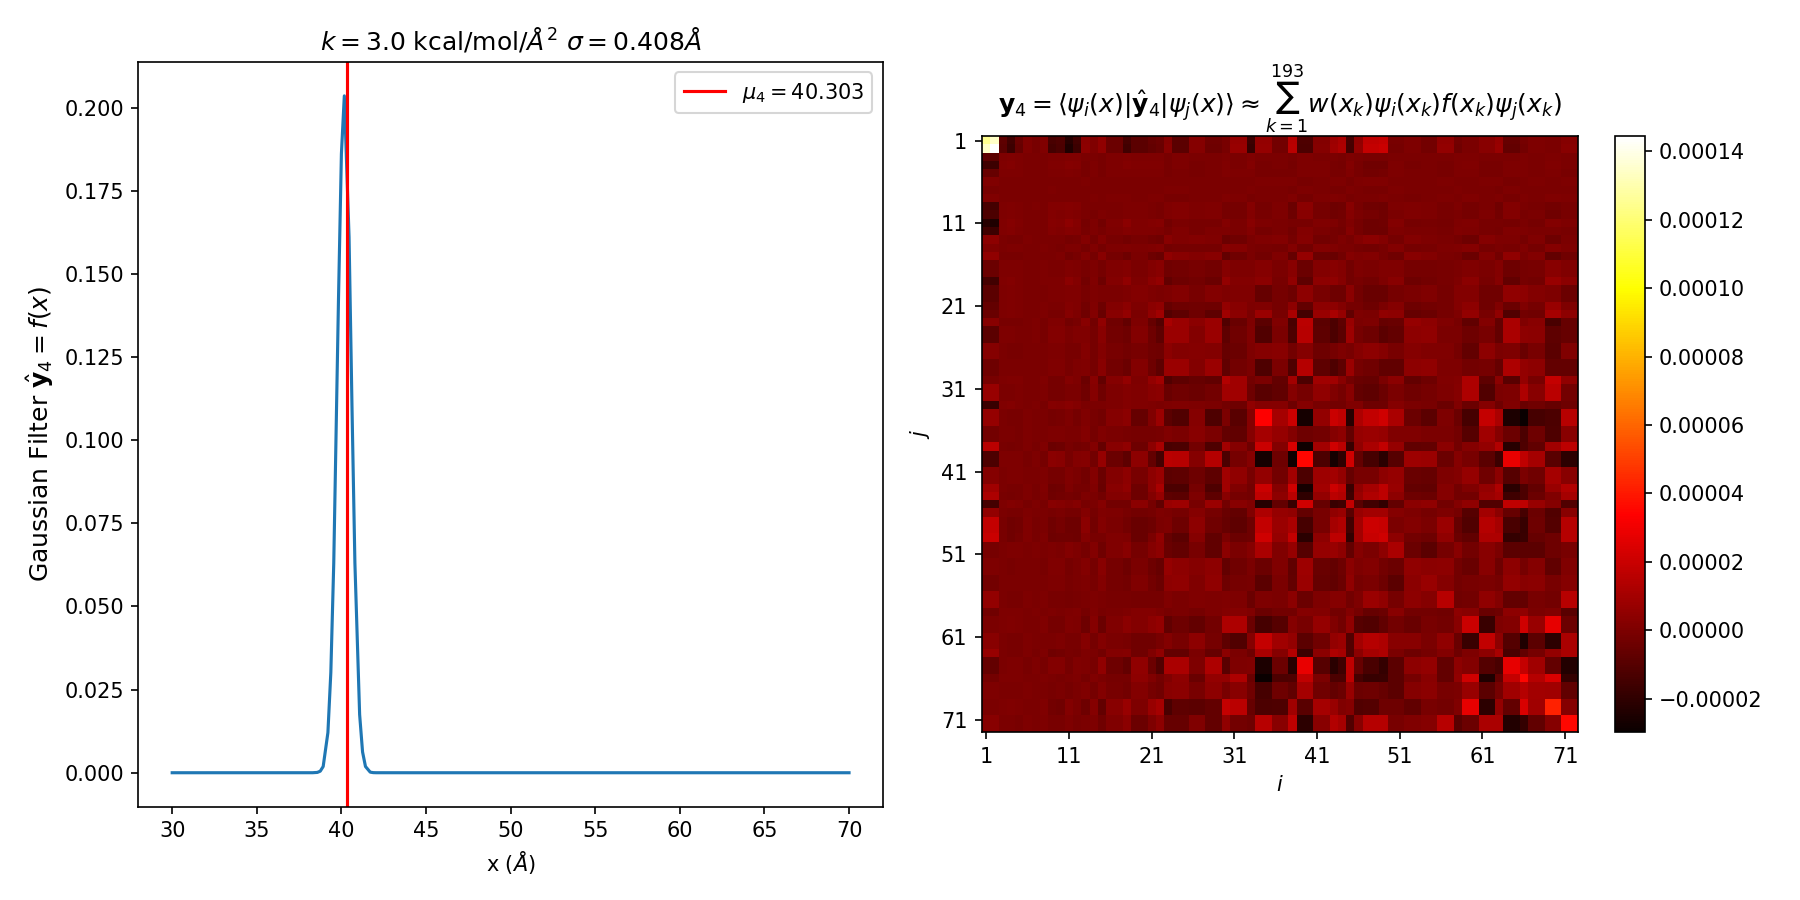
\includegraphics[scale=0.25]{ch2/photon_operator_y3.png}   
\end{center}
\begin{equation}
        \left< \hat{\alpha}_{t_3} \right| 
	= \frac{\left< \hat{\alpha}_{t_2} \right| e^{-\textbf{H}\Delta t} \textbf{y}_3}{\norm{\left< \hat{\alpha}_{t_2} \right| e^{-\textbf{H}\Delta t} \textbf{y}_3}} 
	= \frac{1}{\norm{\alpha_{t_{2}}}} \frac{\left< \alpha_{t_2} \right| e^{-\textbf{H}\Delta t} \textbf{y}_3}{\norm{\left< \hat{\alpha}_{t_2} \right| e^{-\textbf{H}\Delta t} \textbf{y}_3}} 
	= \frac{1}{\norm{\alpha_{t_3}}} \left< \alpha_{t_3} \right|
\end{equation}
where
\begin{equation}
        \norm{\alpha_{t_3}} = \norm{\alpha_{t_{2}}} \norm{\left< \hat{\alpha}_{t_2} \right| e^{-\textbf{H}\Delta t} \textbf{y}_3} 
        = \norm{\left < \hat{\alpha}_{t_{0}} \right| e^{-\textbf{H}\Delta t} \textbf{y}_1} \norm{\left< \hat{\alpha}_{t_1} \right| e^{-\textbf{H}\Delta t} \textbf{y}_2} \norm{\left < \hat{\alpha}_{t_{2}} \right| e^{-\textbf{H}\Delta t} \textbf{y}_3}    
\end{equation}
\begin{center}
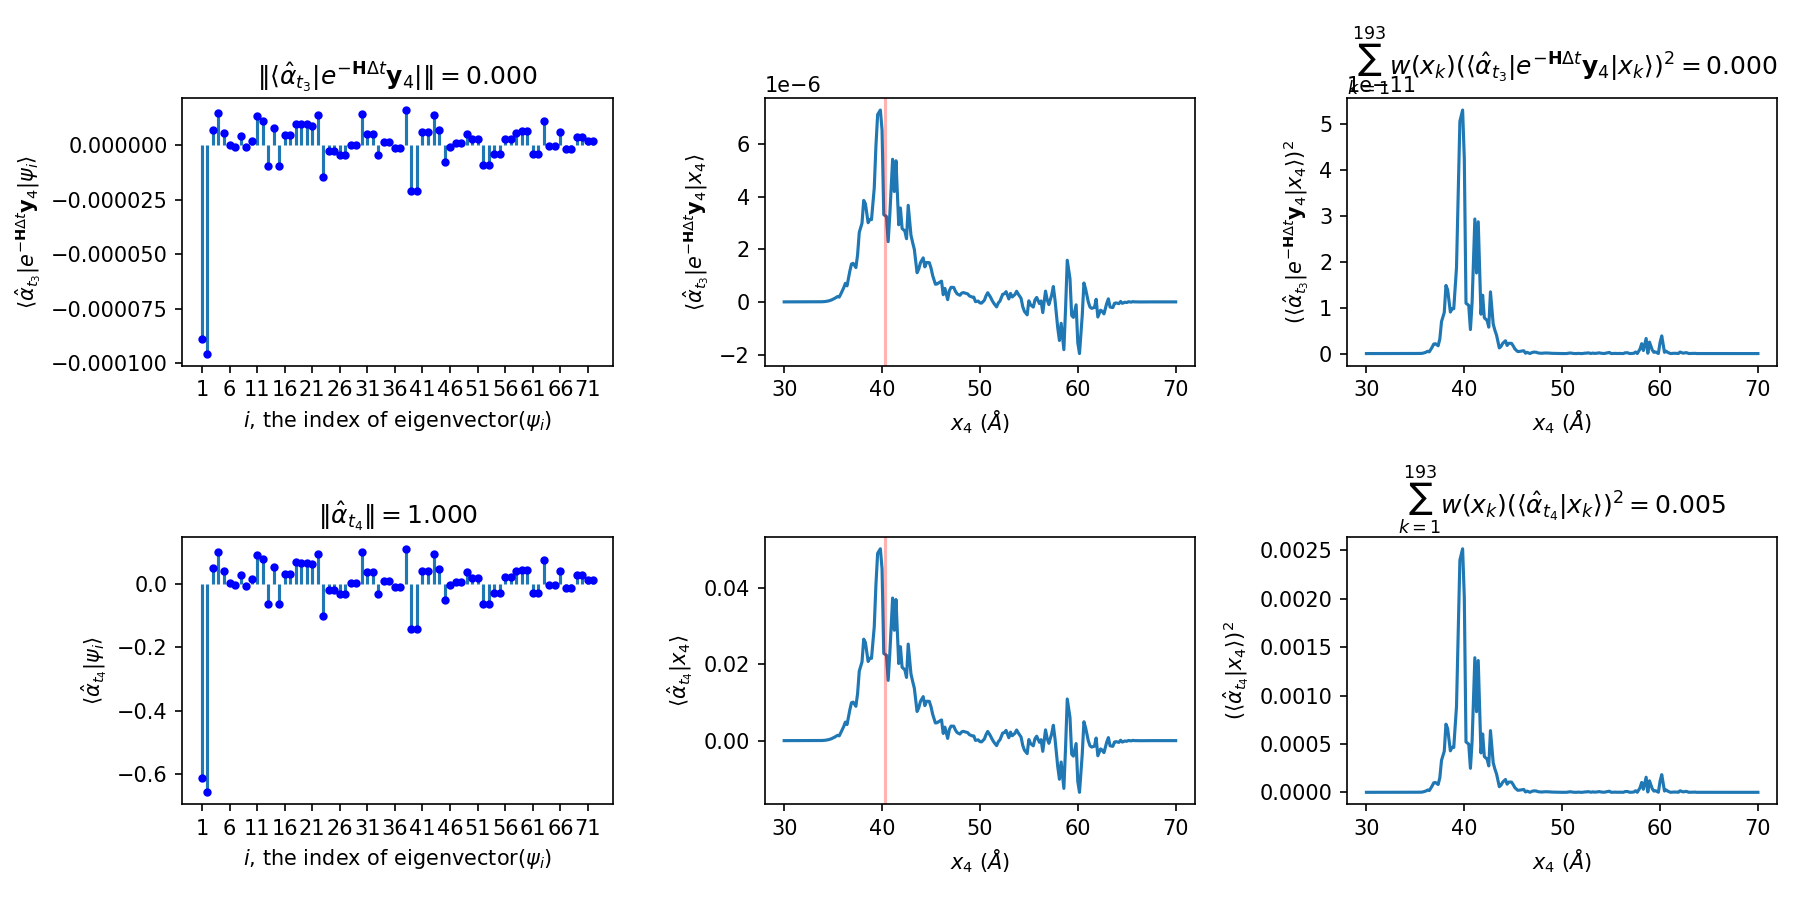
\includegraphics[scale=0.4]{ch2/alpha_3.png}
\end{center}
\end{definition}

\begin{definition}[$\left< \hat{\alpha}_{t_3}| e^{-\textbf{H}\Delta t} \right|$]
The probability meaning is 
\begin{align*}
        (\left< \hat{\alpha}_{t_3}| e^{-\textbf{H}\Delta t} | x_4 \right>)^2 = \int p(x_3 | y_1, y_2, y_3) p(x_4|x_3) dx_4  
\end{align*}
\begin{center}
        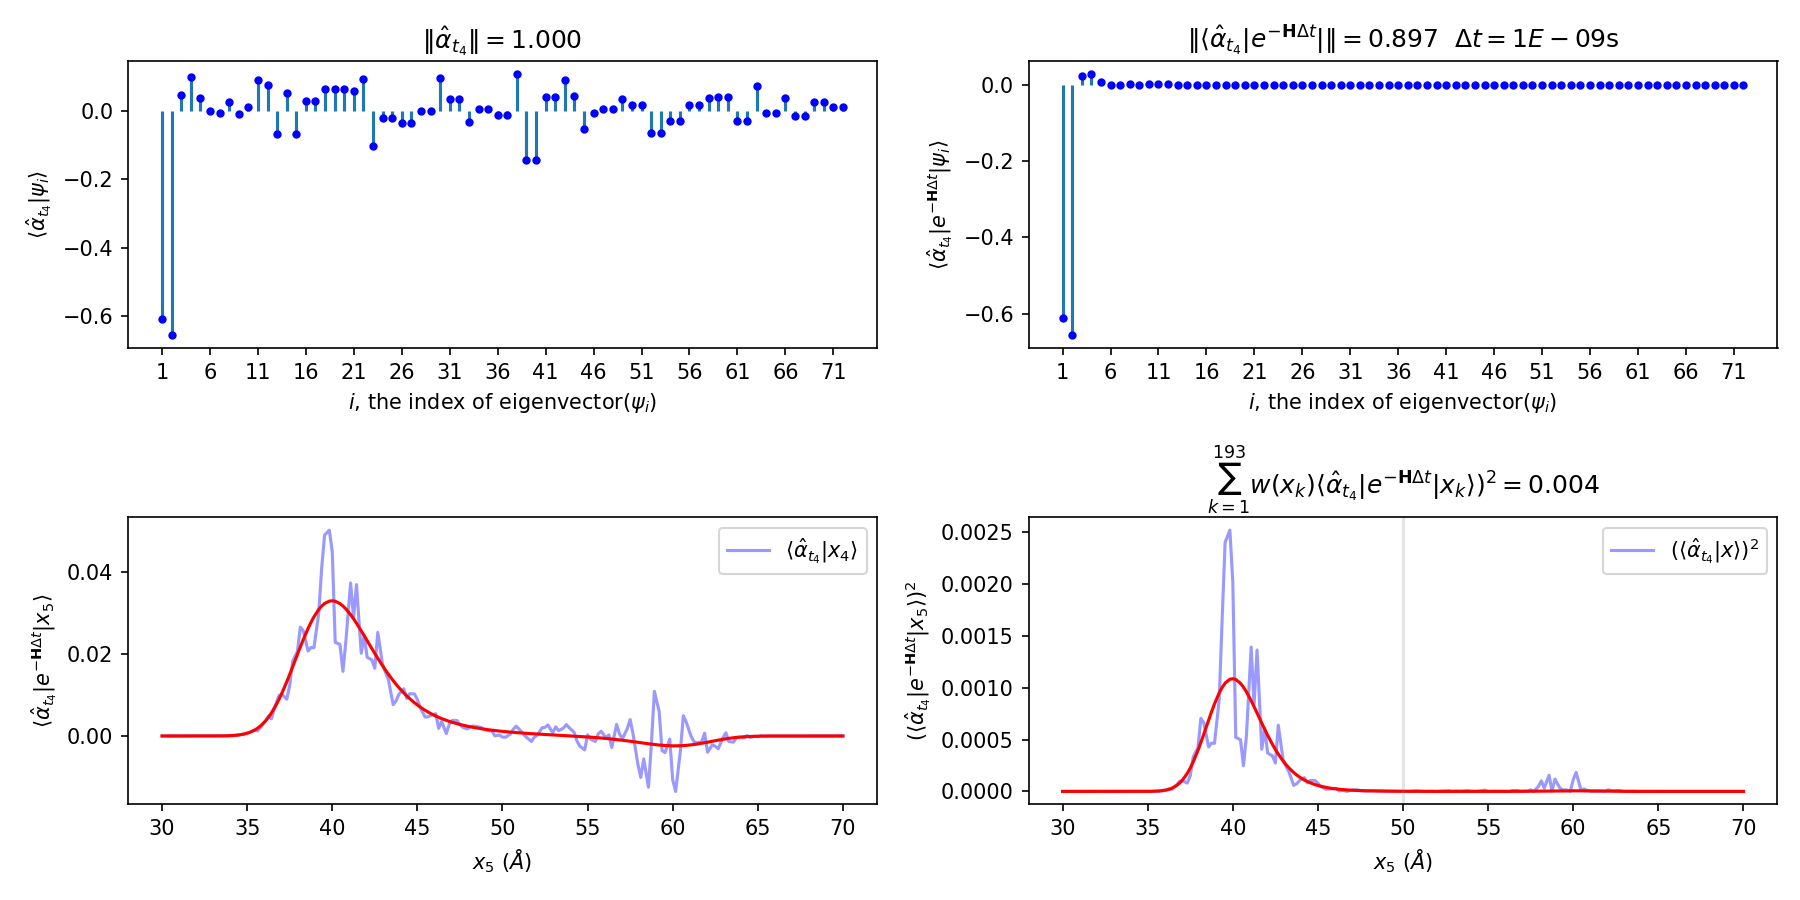
\includegraphics[scale=0.4]{ch2/alphat3_expdt.png}   
\end{center}
\end{definition}

\subsection{alpha-t4}
\begin{definition}[$\left< \hat{\alpha}_{t_4}\right|$]
\begin{equation}
        \left< \alpha_{t_4} \right| = \left< \alpha_{t_3} \right| e^{-\textbf{H}\Delta t} \textbf{y}_4
\end{equation}
\begin{center}
        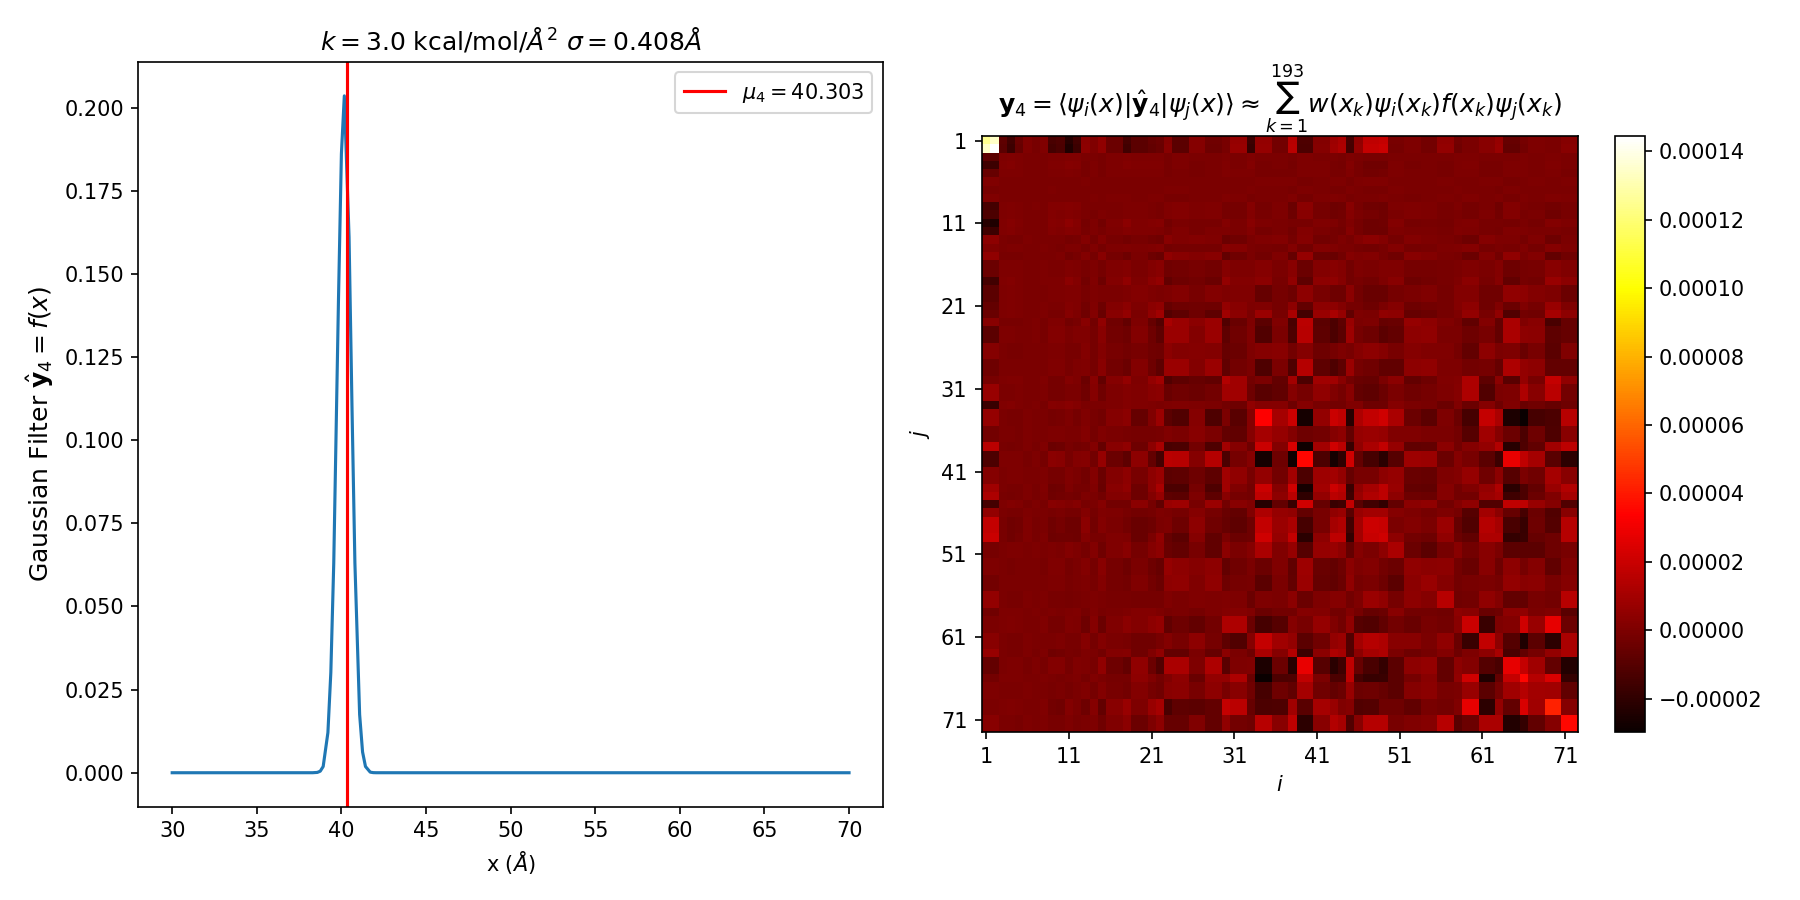
\includegraphics[scale=0.25]{ch2/photon_operator_y4.png}   
\end{center}
\begin{equation}
        \left< \hat{\alpha}_{t_4} \right| 
	= \frac{\left< \hat{\alpha}_{t_3} \right| e^{-\textbf{H}\Delta t} \textbf{y}_4}{\norm{\left< \hat{\alpha}_{t_3} \right| e^{-\textbf{H}\Delta t} \textbf{y}_4}} 
        = \frac{1}{\norm{\alpha_{t_{3}}}} \frac{\left< \alpha_{t_3} \right| e^{-\textbf{H}\Delta t} \textbf{y}_4}{\norm{\left< \hat{\alpha}_{t_3} \right| e^{-\textbf{H}\Delta t} \textbf{y}_4}} 
        = \frac{1}{\norm{\alpha_{t_4}}} \left< \alpha_{t_4} \right|
\end{equation}
where
\begin{equation}
\begin{split}
        \norm{\alpha_{t_4}} &= \norm{\alpha_{t_{3}}} \norm{\left< \hat{\alpha}_{t_3} \right| e^{-\textbf{H}\Delta t} \textbf{y}_4}\\
        &= \norm{\left< \hat{\alpha}_{t_{0}} \right| e^{-\textbf{H}\Delta t} \textbf{y}_1} \norm{\left< \hat{\alpha}_{t_1} \right| e^{-\textbf{H}\Delta t} \textbf{y}_2} \norm{\left < \hat{\alpha}_{t_{2}} \right| e^{-\textbf{H}\Delta t} \textbf{y}_3} \norm{\left < \hat{\alpha}_{t_{3}} \right| e^{-\textbf{H}\Delta t} \textbf{y}_4}
\end{split}
\label{eq:alphat4}
\end{equation}
\begin{center}
        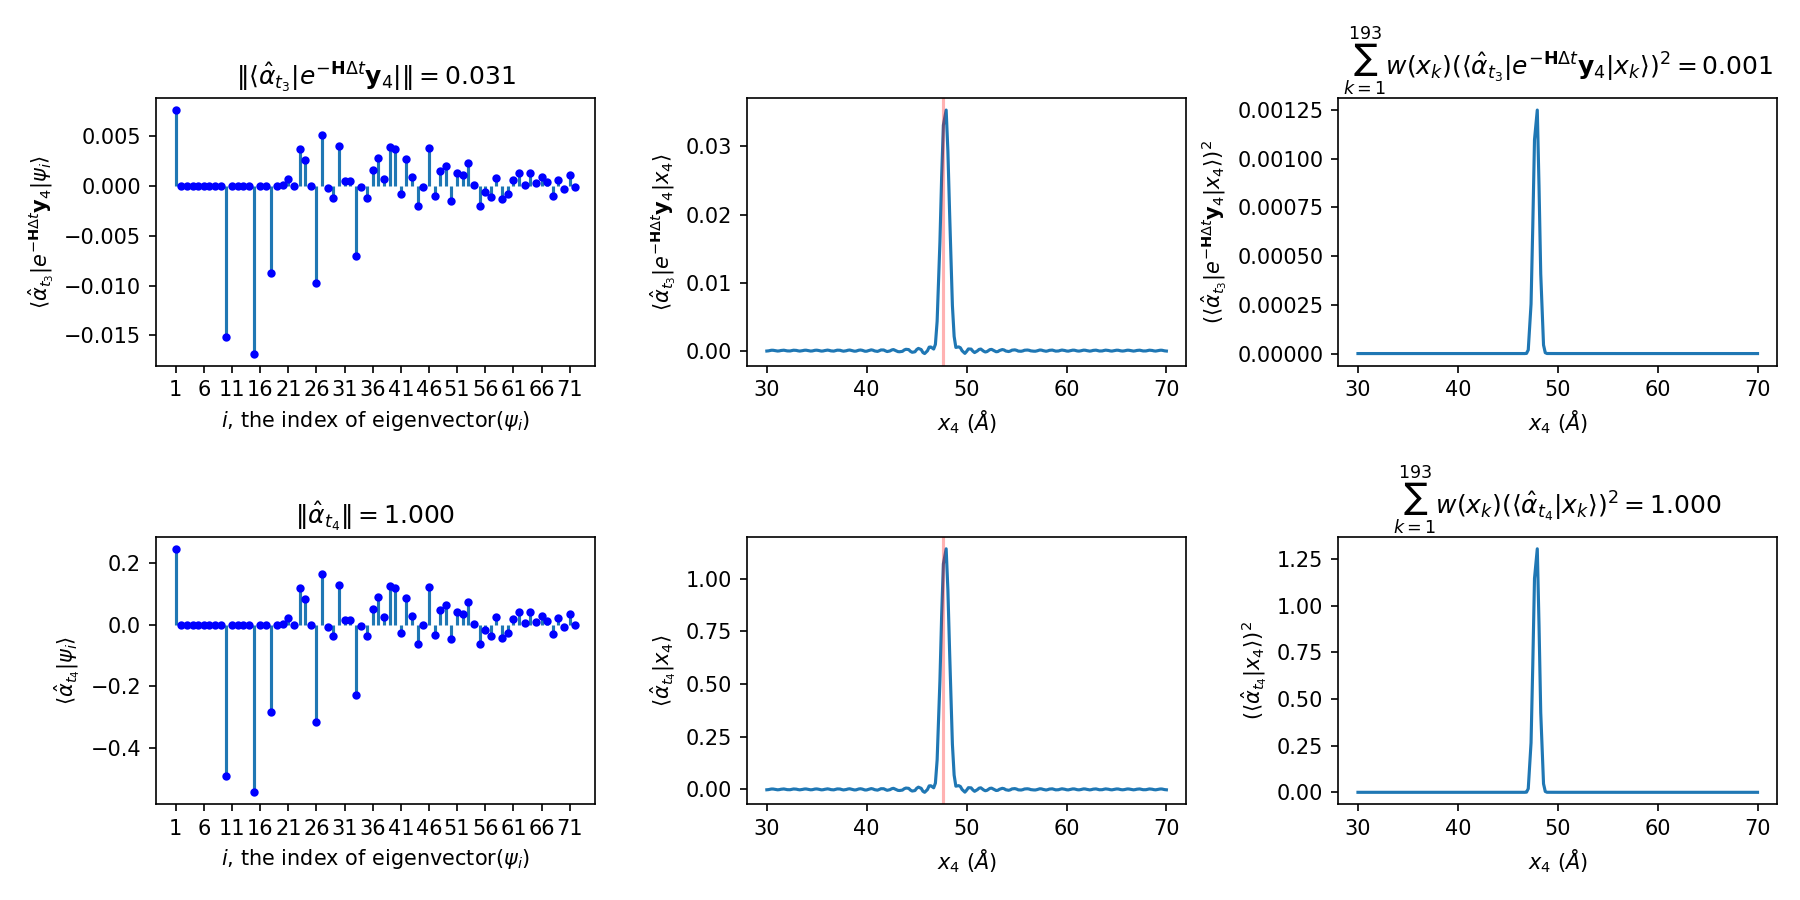
\includegraphics[scale=0.4]{ch2/alpha_4.png}
\end{center}
\end{definition}

\begin{definition}[$p(x_4|\textbf{y})$]
\begin{equation}
        \left(\left<  \hat{\alpha}_{t_4} | x \right>\right)^2 = p(x_4|y_1,y_2,y_3,y_4)
\end{equation}
\begin{center}
        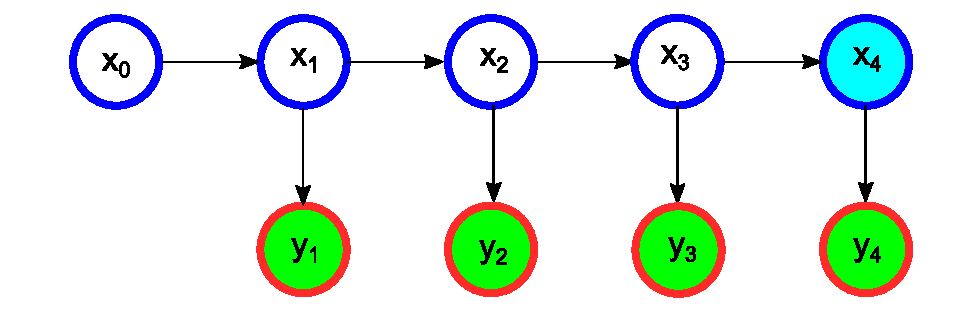
\includegraphics[scale=0.7]{ch2/alpha_hat_4_graphical.pdf}
\end{center}
\begin{center}
        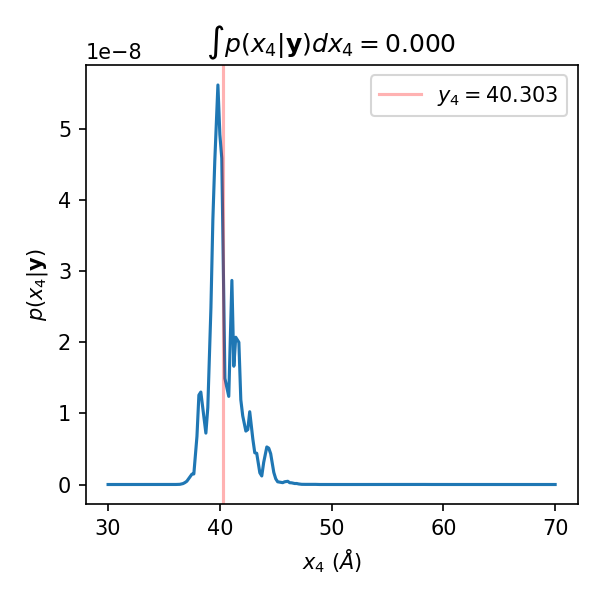
\includegraphics[scale=0.5]{ch2/posterior_4.png}
\end{center}       
\end{definition}

\section{Scaling Factor}
\begin{definition}[$\norm{\alpha_{t_{\tau}}}^2$]
\begin{equation}
        \left(\left< \hat{\alpha}_{t_{\tau}} | x \right>\right)^2 = p(x_{\tau}|y_1,\cdots,y_{\tau})  = 
        \frac{p(y_1,\cdots,y_{\tau}, x_{\tau})}{p(y_1,\cdots,y_{\tau})} =
        \frac{\left(\left< \alpha_{t_{\tau}} | x \right>\right)^2}{\norm{\alpha_{t_{\tau}}}^2} 
\end{equation}
Therefore,
\begin{equation}
        \norm{\alpha_{t_{\tau}}}^2 = p(y_1,\cdots,y_{\tau}) 
\end{equation}
\begin{center}
        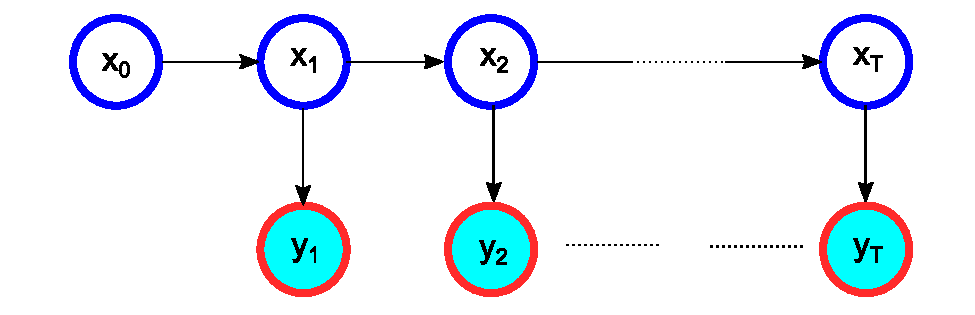
\includegraphics[scale=0.6]{ch2/norm_example.pdf}
\end{center}
Furthermore, the likelihood function $p(\textbf{y})$
\begin{equation}
        \norm{\alpha_{t_{T}}}^2 =  p(y_1,\cdots,y_T) = p(\textbf{y})
\end{equation}
\end{definition}

\begin{definition}[Scaling factor $c_i$]
From eq(\ref{eq:alphat4}), we know
\begin{equation}
        \norm{\alpha_{t_{\tau}}} = \prod_{i=1}^{\tau} \norm{\left < \hat{\alpha}_{t_{i-1}} \right| e^{-\textbf{H}\Delta t} \textbf{y}_i} = \prod_{i=1}^{\tau} c_i
\end{equation}
To understand the probability meaning, we first do 
\begin{equation}
        \left(\left < \hat{\alpha}_{t_{i-1}} | e^{-\textbf{H}\Delta t} \textbf{y}_{i} | x \right>\right)^2 = p(x_{i},y_{i}|y_1,\cdots,y_{i-1})   
\end{equation}
\begin{equation}
\begin{split}       
        \norm{\left < \hat{\alpha}_{t_{i-1}} | e^{-\textbf{H}\Delta t} \textbf{y}_{i} \right|}^2 &= \int w(x) \left(\left < \hat{\alpha}_{t_{i-1}} | e^{-\textbf{H}\Delta t} \textbf{y}_{i} | x \right>\right)^2 dx \\
        &= \int p(x_{i},y_{i}|y_1,\cdots,y_{i-1}) dx = p(y_i | y_1,\cdots,y_{i-1})
\end{split}
\end{equation}
Therefore, the probability meaning of $c_i$ is 
\begin{equation}
        c_i^2 = p(y_i | y_1,\cdots,y_{i-1})
\label{eq:scalefactor} 
\end{equation}
Furthermore, the following is consistent
\begin{equation}
        \left(\left < \hat{\alpha}_{t_i} | x \right>\right)^2 =  p(x_{i}|y_1,\cdots,y_{i})  = 
        \frac{p(x_{i},y_{i}|y_1,\cdots,y_{i-1})}{p(y_i | y_1,\cdots,y_{i-1})} = \frac{  \left(\left < \hat{\alpha}_{t_{i-1}} | e^{-\textbf{H}\Delta t} \textbf{y}_{i} | x \right>\right)^2 }{ \norm{\left < \hat{\alpha}_{t_{i-1}} | e^{-\textbf{H}\Delta t} \textbf{y}_{i} \right|}^2 } 
\end{equation}
\end{definition}

\begin{definition}[Likelihood function]
The likelihood function $p(\textbf{y})$
\begin{equation}
        p(\textbf{y}) = p(y_1,\cdots,y_T) = \norm{\alpha_{t_{T}}}^2 = \prod_{i=1}^{T} \norm{\left < \hat{\alpha}_{t_{i-1}} \right| e^{-\textbf{H}\Delta t} \textbf{y}_i}^2 = \prod_{i=1}^{T} c_i^2
\end{equation}              
\end{definition}

\begin{definition}[Log likelihood function]
\begin{equation}
        l(\theta) = \ln{(p(\textbf{y}))} = \ln{(\prod_{i=1}^{T} c_i^2)} = 2\sum_{i=1}^{T} \ln{c_i}  
\end{equation}
\begin{center}
        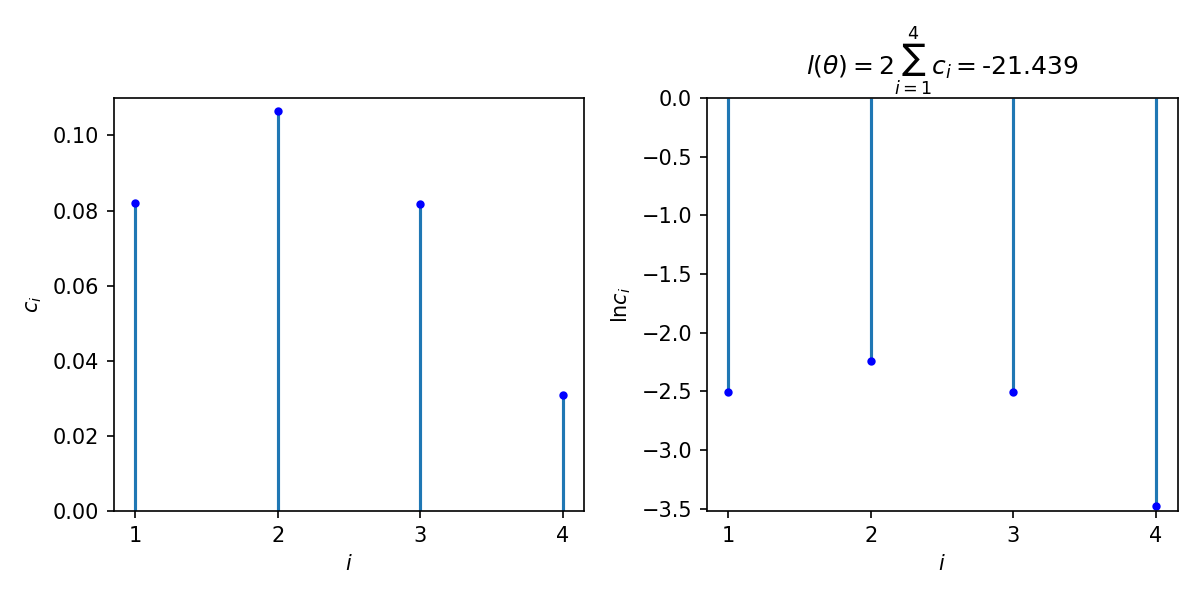
\includegraphics[scale=0.45]{ch2/likelihood_example.png}
\end{center}
\end{definition}

\section{Backward algorithm}
\subsection{Probability Meaning}
First, the $ \left<x|\beta_{t_{\tau}} \right>$ is the probability amplitude of emitting a partial sequence of outputs $(y_{\tau+1},\cdots,y_{T})$ given that the system starts in state $x_{\tau}$. That is,
\begin{equation}
        (\left<x|\beta_{t_{\tau}} \right>)^2 = p(y_{\tau+1},\cdots,y_{T}|x_{\tau})
\end{equation}
For example, $(\left<x|\beta_{2} \right>)^2 = p(y_3, y_4|x_2)$
\begin{center}
        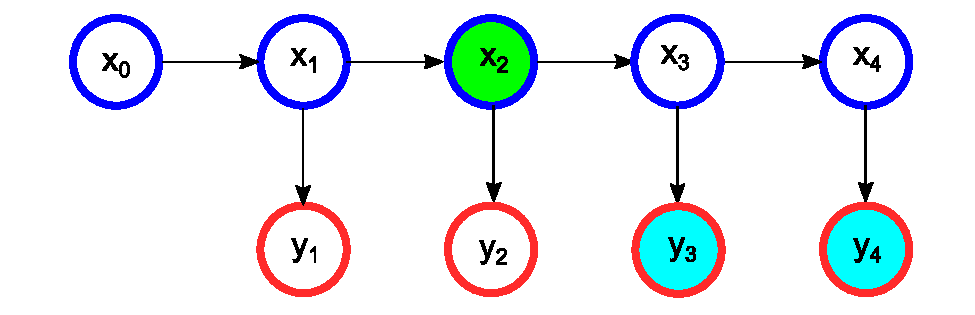
\includegraphics[scale=0.6]{ch2/beta_example.pdf}
\end{center}

\subsection{beta-4}
\begin{definition}[$\left | \beta_{t_4} \right > $]
As you can see in Definition(\ref{specialposterior}), we let
\begin{equation}\label{beta4}
        \left<x|\beta_{t_4} \right>=1~~\forall x 
\end{equation}
and we want to find $\left|\beta_{t_4} \right> $ which is in eigenspace
\begin{equation}
        \left|\beta_{t_4} \right> = \begin{bmatrix}
                \left< \psi_1|\beta_{t_4} \right> \\ \left< \psi_2|\beta_{t_4} \right> \\ \vdots \\ 
                \left< \psi_{72}|\beta_{t_4} \right>
        \end{bmatrix} 
\end{equation}
where
\begin{equation}\label{beta4dotproduct}
        \left< \psi_j | \beta_{t_4} \right> = \int w(x) \psi_j(x)  \left<x|\beta_{t_4} \right> dx
        = \int w(x) \psi_j(x) dx \approx \sum_{i=1}^{193} w(x_i) \psi_j(x_i).
\end{equation}
We substitute eq(\ref{beta4}) into eq(\ref{beta4dotproduct}).
\begin{center}
        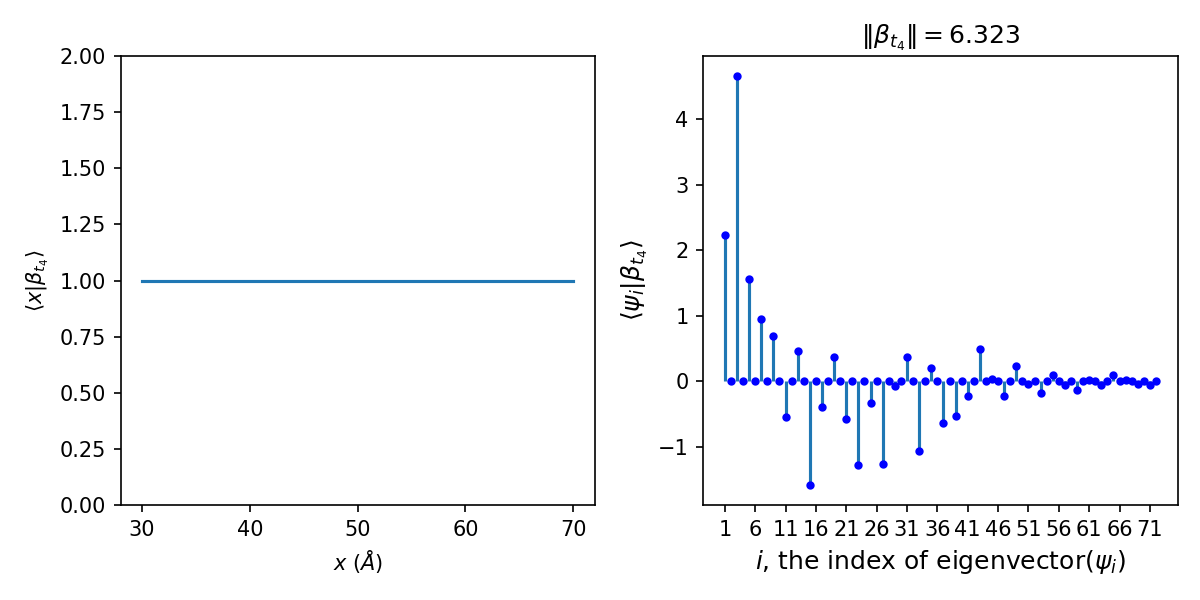
\includegraphics[scale=0.45]{ch2/beta_4.png}
\end{center}
\end{definition}

\subsection{beta-3}
\begin{definition}[$ \left| \beta_{t_3} \right>$]
\begin{equation}
        \left|\beta_{t_3}  \right> =  \left| e^{-\textbf{H}\Delta t} \textbf{y}_4 |\beta_{t_4} \right>
\end{equation}
The probability meaning is
\begin{equation}
   \left( \left<x_3 |\beta_{t_3}  \right> \right)^2 = p(y_4 | x_3) = \int p(x_4 | x_3) p(y_4 | x_4) dx_4
\end{equation}
\begin{center}
        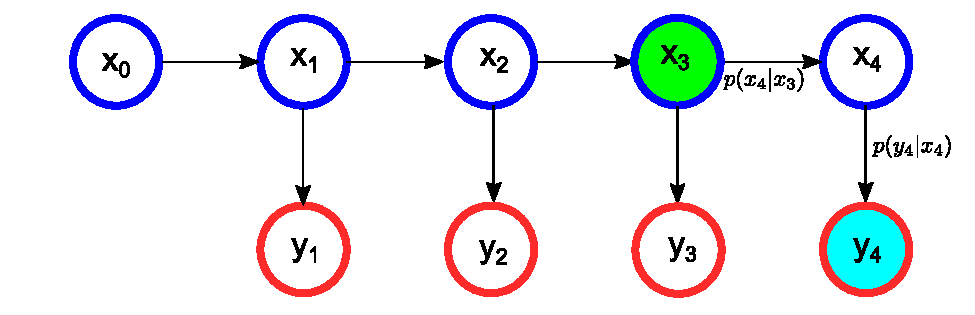
\includegraphics[scale=0.6]{ch2/beta_3_graphical.pdf}
\end{center}
\begin{center}
        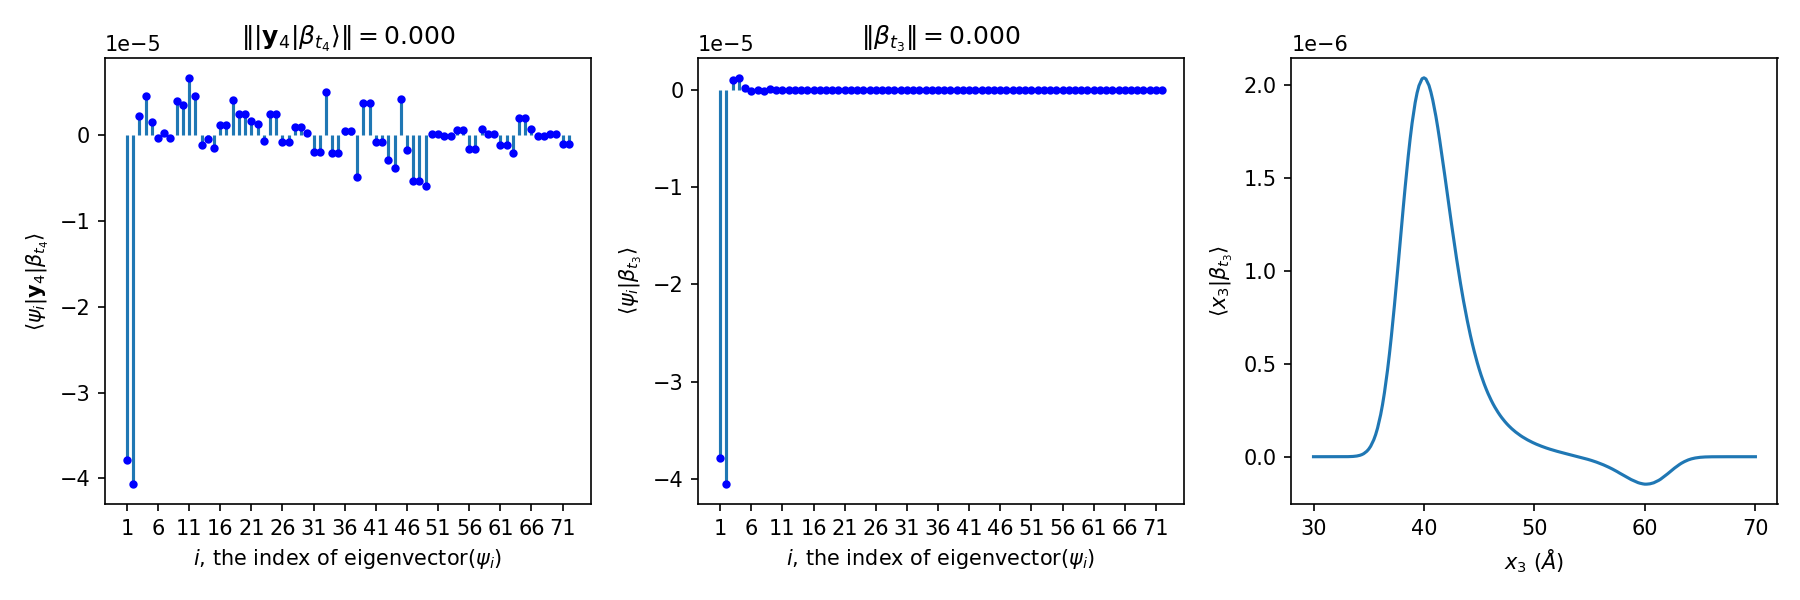
\includegraphics[scale=0.45]{ch2/beta_3.png}
\end{center}
\end{definition}

\begin{definition}[$\left| \hat{\beta}_{t_3} \right>$]
\begin{equation}
        \left| \hat{\beta}_{t_{3}} \right> = \frac{ \left| \beta_{t_{3}} \right> }{ c_4 }
\end{equation}
where $c_4$ is the scaling factor computed in the forward part, as you can see in eq(\ref{eq:scalefactor}), and 
the probability meaning is
\begin{equation}
        \left(\left<x_3|\hat{\beta}_{t_{3}} \right>\right)^2 = \frac{p(y_4|x_3)}{p(y_4|y_1,y_2,y_3)} 
        =  \frac{ (\left<x_3|\beta_{t_{3}} \right>)^2 }{ c_4^2 }
\end{equation}
\begin{center}
        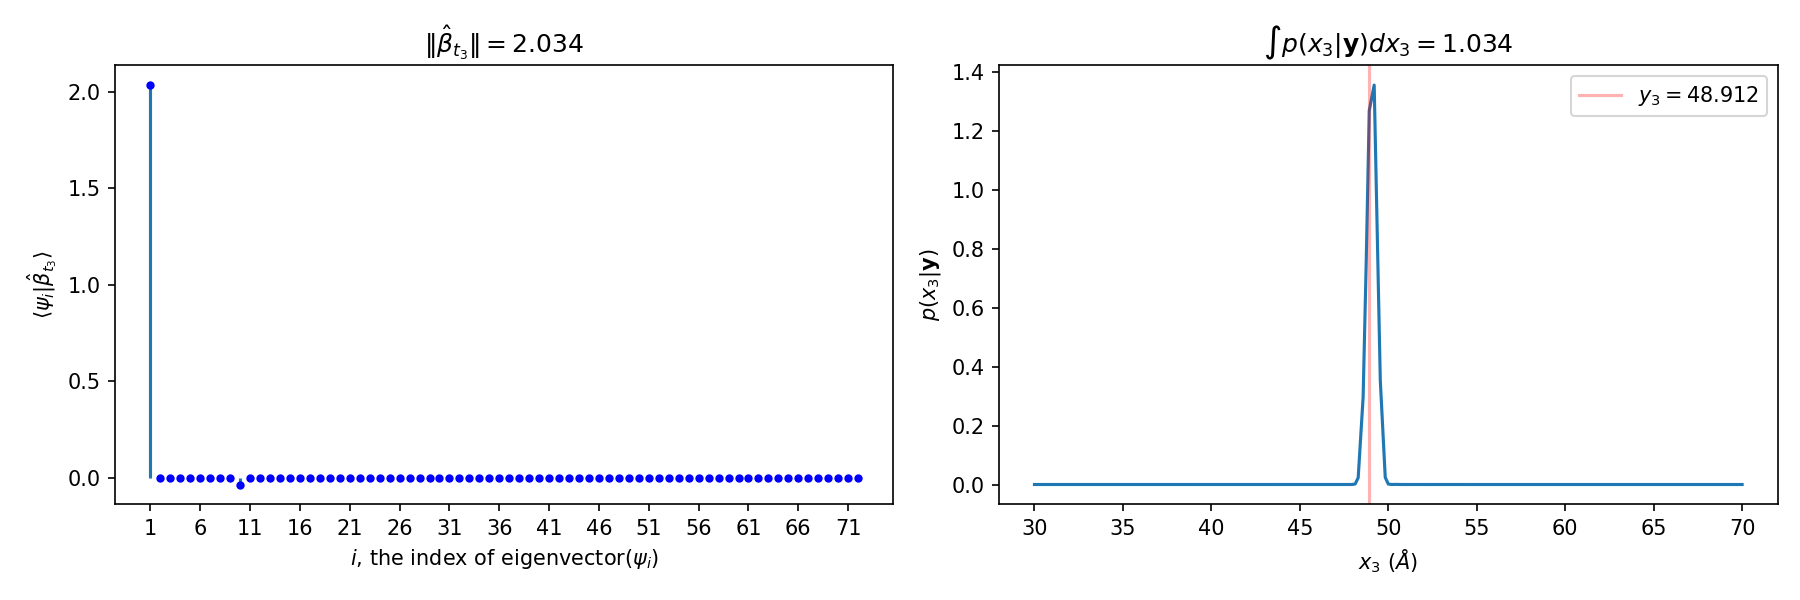
\includegraphics[scale=0.45]{ch2/beta_3_hat.png}
\end{center}
\begin{equation}
        p(x_3|\textbf{y}) = (\left<\hat{\alpha}_{t_{3}}|x \right>)^2 \left(\left<x|\hat{\beta}_{t_{3}} \right>\right)^2
\end{equation} 
\end{definition}

\subsection{beta-2}
\begin{definition}[$\left| \beta_{t_2} \right>$]
\begin{equation}
        \left|\beta_{t_2}  \right> =  \left| e^{-\textbf{H}\Delta t} \textbf{y}_3 |\beta_{t_3} \right>
\end{equation}
The probability meaning is
\begin{equation}
           \left( \left<x_2 |\beta_{t_2}  \right> \right)^2 = p(y_3, y_4 | x_2)
\end{equation}
\begin{center}
        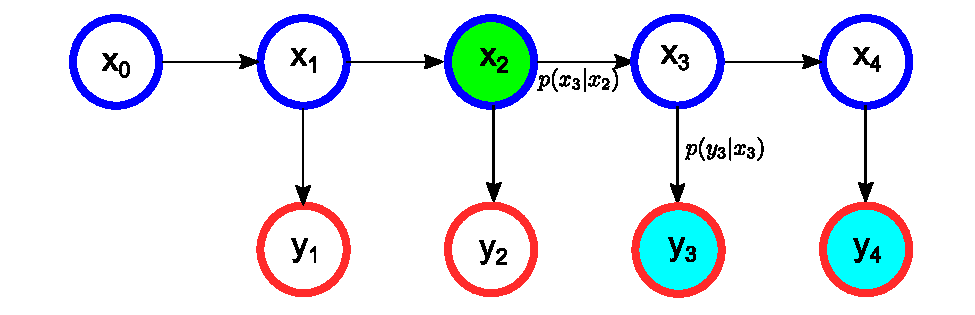
\includegraphics[scale=0.6]{ch2/beta_2_graphical.pdf}
\end{center}       
\end{definition}

\begin{definition}[$\left| \hat{\beta}_{t_2} \right>$]
\begin{equation}
        \left|\hat{\beta}_{t_2}  \right> =  \frac{\left| e^{-\textbf{H}\Delta t} \textbf{y}_3 |\hat{\beta}_{t_3} \right>}{c_3}
\end{equation}
where $c_3$ is the scaling factor computed in the forward part, as you can see in eq(\ref{eq:scalefactor}), and 
the probability meaning is
\begin{equation}
        \left(\left<x_2|\hat{\beta}_{t_{2}} \right>\right)^2 = \frac{p(y_3, y_4|x_2)}{p(y_3|y_1,y_2)} 
        =  \frac{ (\left<x_2|\beta_{t_{2}} \right>)^2 }{ c_3^2 }
\end{equation}
\begin{center}
        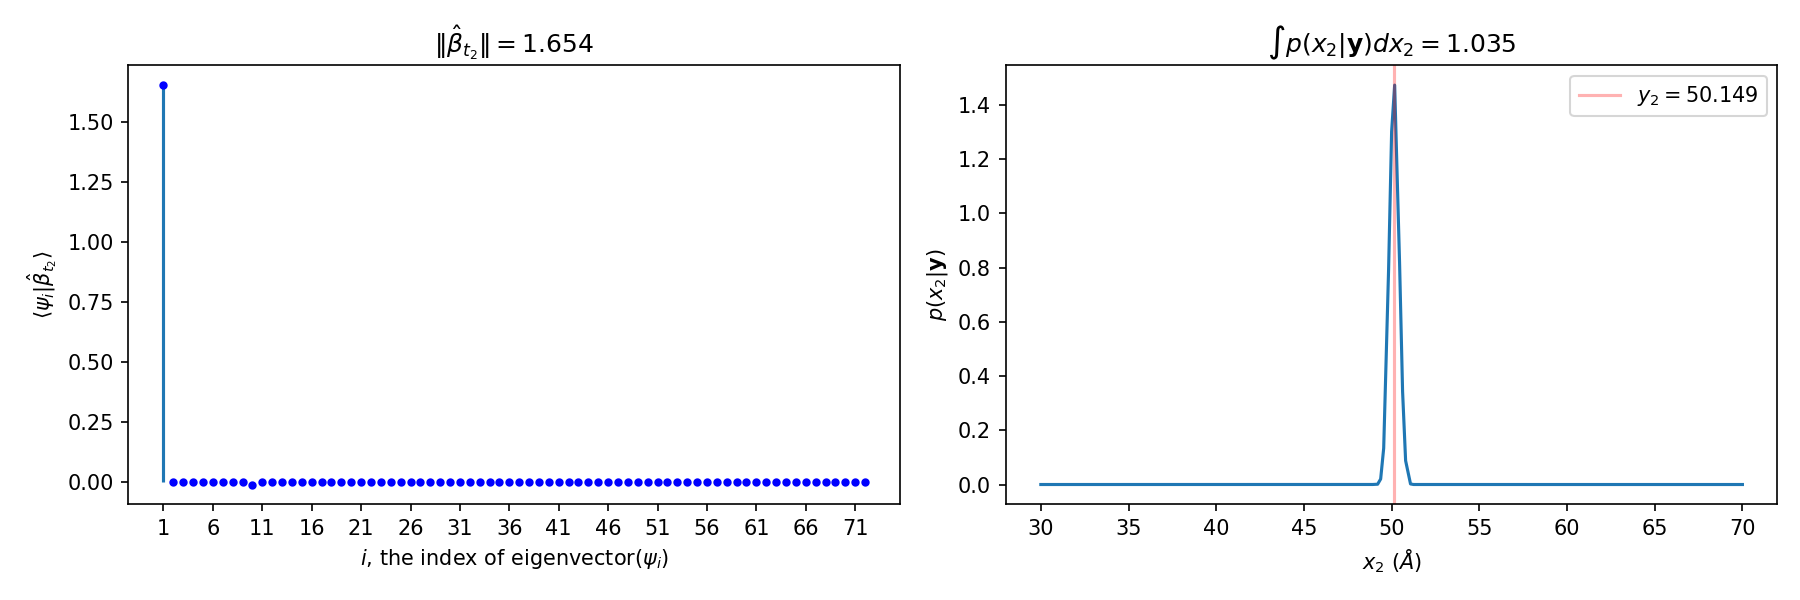
\includegraphics[scale=0.45]{ch2/beta_2_hat.png}
\end{center}
\begin{equation}
        p(x_2|\textbf{y}) = (\left<\hat{\alpha}_{t_{2}}|x \right>)^2 \left(\left<x|\hat{\beta}_{t_{2}} \right>\right)^2
\end{equation} 
\end{definition}

\subsection{beta-1}
\begin{definition}[$\left| \beta_{t_1} \right>$]
\begin{equation}
        \left|\beta_{t_1}  \right> =  \left| e^{-\textbf{H}\Delta t} \textbf{y}_2 |\beta_{t_2} \right>
\end{equation}
The probability meaning is
\begin{equation}
           \left( \left<x_1 |\beta_{t_1}  \right> \right)^2 = p(y_2, y_3, y_4 | x_1)
\end{equation}
\begin{center}
        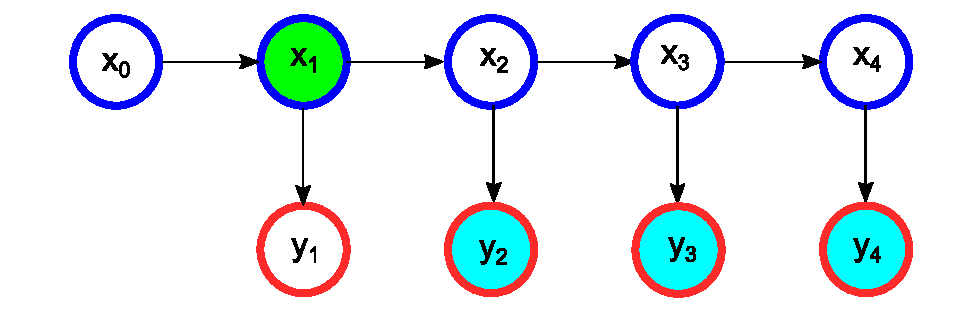
\includegraphics[scale=0.6]{ch2/beta_1_graphical.pdf}
\end{center}       
\end{definition}

\begin{definition}[$\left| \hat{\beta}_{t_1} \right>$]
\begin{equation}
        \left|\hat{\beta}_{t_1}  \right> =  \frac{\left| e^{-\textbf{H}\Delta t} \textbf{y}_2 |\hat{\beta}_{t_2} \right>}{c_2}
\end{equation}
where $c_2$ is the scaling factor computed in the forward part, as you can see in eq(\ref{eq:scalefactor}), and 
the probability meaning is
\begin{equation}
        \left(\left<x_1|\hat{\beta}_{t_1} \right>\right)^2 = \frac{p(y_2, y_3, y_4|x_1)}{p(y_2|y_1)} 
        =  \frac{ (\left<x_1|\beta_{t_1} \right>)^2 }{ c_2^2 }
\end{equation}
\begin{center}
        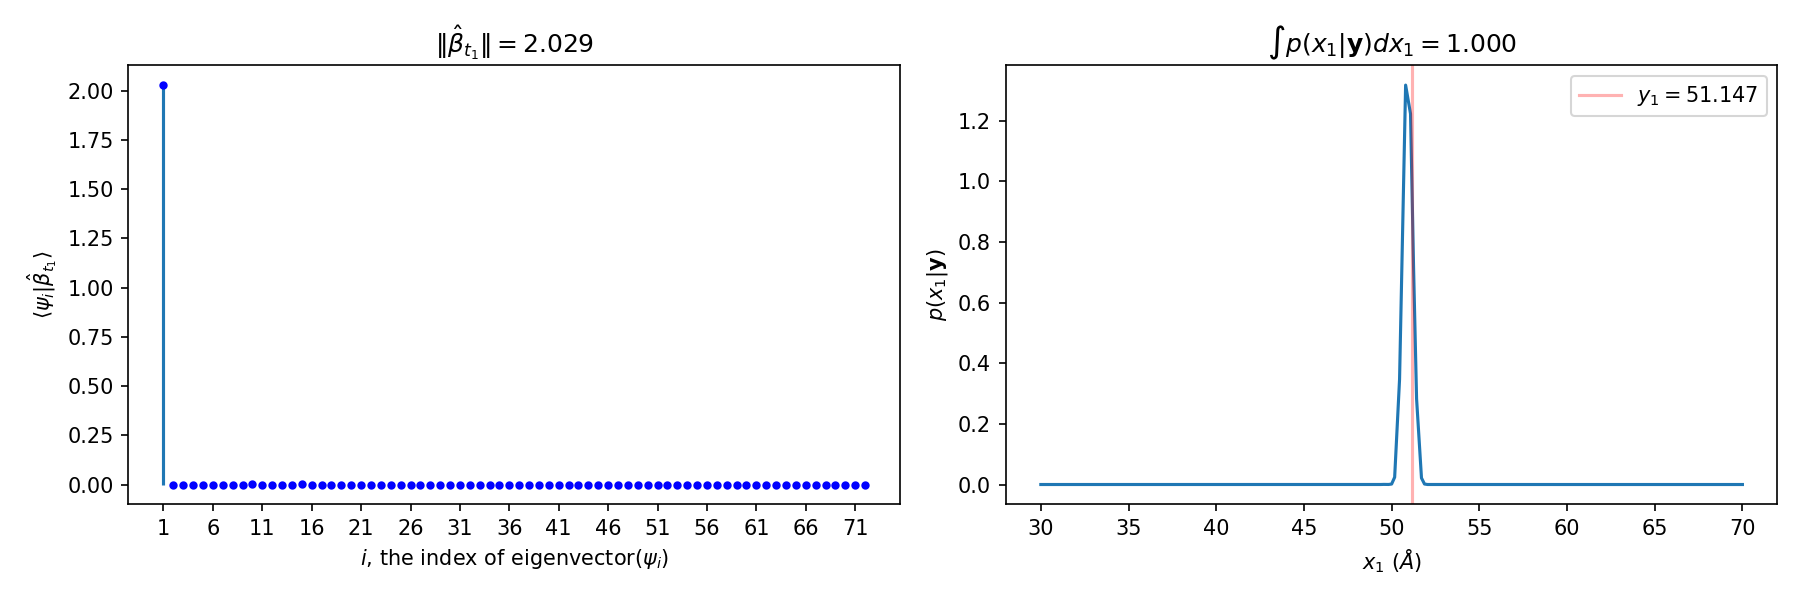
\includegraphics[scale=0.45]{ch2/beta_1_hat.png}
\end{center}
\begin{equation}
        p(x_1|\textbf{y}) = (\left<\hat{\alpha}_{t_{1}}|x \right>)^2 \left(\left<x|\hat{\beta}_{t_{1}} \right>\right)^2
\end{equation} 
\end{definition}

\section{Posterior probability}
\begin{definition}[$p(x_{\tau}|\textbf{y})$] 
The posterior probability on a particular state node $x_{\tau}$, where $\textbf{y}$ is all emission sequence
\begin{align*}
        \textbf{y} = (y_1,\cdots,y_T)
\end{align*} 
\end{definition}
\noindent We focus on a particular state node $x_{\tau}$ and ask to calculate its posterior probability, $p(x_{\tau}| \textbf{y})$. And by Bayes' theorem,
\begin{equation}
p(x_{\tau} | \textbf{y}) = \frac{p(\textbf{y}|x_{\tau}) p(x_{\tau})}{p(\textbf{y})}
\end{equation}
Then, conditioning on $x_{\tau}$ and use conditional independence:
\begin{equation}
p(x_{\tau} | \textbf{y}) = \frac{p(y_1,\cdots,y_{\tau}|x_{\tau}) p(y_{\tau+1},\cdots,y_T|x_{\tau}) p(x_{\tau})}{p(\textbf{y})}
\end{equation}
Regroup the terms
\begin{equation}
\begin{split}
p(x_{\tau} | \textbf{y}) &= \frac{p(y_1,\cdots,y_{\tau},x_{\tau}) p(y_{\tau+1},\cdots,y_T|x_{\tau})}{p(\textbf{y})}\\
&=\frac{(\left<\alpha_{t_{\tau}}|x \right>)^2 (\left<x|\beta_{t_{\tau}} \right>)^2 }{p(\textbf{y})}
\end{split}
\end{equation}

\begin{definition}[Special case: $p(x_T|\textbf{y})$]
\label{specialposterior}
\begin{equation}
p(x_T | \textbf{y}) =\frac{(\left<\alpha_{t_T}|x \right>)^2 (\left<x|\beta_{t_T} \right>)^2 }{p(\textbf{y})}
\end{equation}
where
\begin{align}
        (\left<\alpha_{t_T}|x \right>)^2 &=  p(y_1,\cdots,y_T,x_T) = p(\textbf{y}, x_T) \\
        (\left<x|\beta_{t_T} \right>)^2 &= p(y_{T+1}|x_T)\text{~~~Some problem here!}
\end{align}
As you can see, we can not define $\left<x|\beta_{t_T} \right>$ because there is no $y_{T+1}$. Also, we notice
\begin{align*}
        p(x_T | \textbf{y}) = \frac{(\left<\alpha_{t_T}|x \right>)^2}{p(\textbf{y})} = \frac{p(\textbf{y}, x_T)}{p(\textbf{y})}
\end{align*}
Therefore, we just let
\begin{equation}
        \left<x|\beta_{t_T} \right>=1~~\forall x
\end{equation}
\end{definition}

\begin{definition}[$p(x_3|\textbf{y})$]
\begin{equation}
        p(x_3|\textbf{y}) = \frac{(\left<\alpha_{t_{3}}|x \right>)^2 (\left<x|\beta_{t_{3}} \right>)^2 }{p(\textbf{y})} 
        = (\left<\hat{\alpha}_{t_{3}}|x \right>)^2 \left(\left<x|\hat{\beta}_{t_{3}} \right>\right)^2
\end{equation}
where
\begin{equation}
        (\left<\hat{\alpha}_{t_{3}}|x \right>)^2 = 
        \frac{p(y_1,y_2,y_3, x_3)}{p(y_1,y_2,y_3)} =
        p(x_3|y_1,y_2,y_3)=
        \frac{\left(\left< \alpha_{t_3} | x \right>\right)^2}{\norm{\alpha_{t_3}}^2}   
\end{equation}
and
\begin{equation}
        \left(\left<x|\hat{\beta}_{t_{3}} \right>\right)^2 = \frac{p(y_4|x_3)}{p(y_4|y_1,y_2,y_3)} 
        =  \frac{ (\left<x|\beta_{t_{3}} \right>)^2 }{ c_4^2 }
\end{equation}
In the last line, we used eq(\ref{eq:scalefactor}).
\begin{center}
        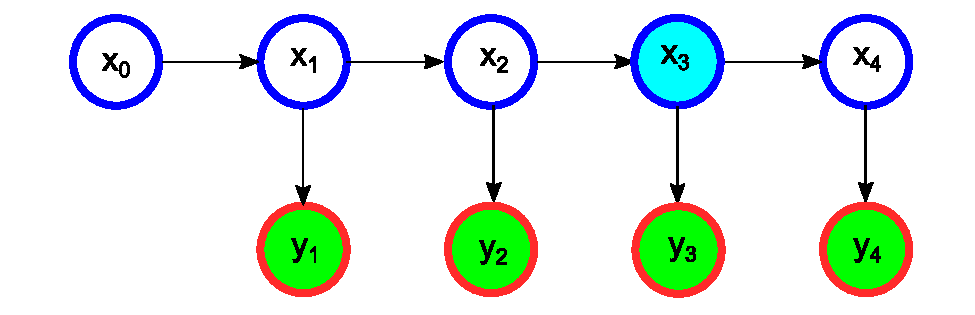
\includegraphics[scale=0.6]{ch2/posterior_3.pdf}
\end{center}   
\end{definition}